\documentclass{article}




\usepackage[preprint]{neurips_2023}








\usepackage[utf8]{inputenc} %
\usepackage[T1]{fontenc}    %
\usepackage[hidelinks]{hyperref}       %
\usepackage{url}            %
\usepackage{booktabs}       %
\usepackage{amsmath}
\usepackage{amsfonts}       %
\usepackage{amsthm}       %
\usepackage{nicefrac}       %
\usepackage{microtype}      %
\usepackage{cleveref}
\usepackage[disable]{todonotes}
\usepackage{xcolor}         %
\usepackage{verbatim}

\theoremstyle{plain}
\newtheorem*{theorem*}{Theorem}
\newtheorem{theorem}{Theorem}[section]
\newtheorem{proposition}[theorem]{Proposition}
\newtheorem{lemma}[theorem]{Lemma}
\newtheorem*{lemma*}{Lemma}
\newtheorem{corollary}[theorem]{Corollary}
\theoremstyle{definition}
\newtheorem{definition}[theorem]{Definition}
\newtheorem{assumption}[theorem]{Assumption}
\theoremstyle{remark}
\newtheorem{remark}[theorem]{Remark}



\newcommand{\fracpartial}[2]{\frac{\partial #1}{\partial  #2}}
\newcommand{\numeq}[1]{\begin{align}#1\end{align}}
\newcommand{\eq}[1]{\begin{align*}#1\end{align*}}
\newcommand{\E}{\mathbb{E}}
\newcommand{\p}{\mathbb{P}}
\newcommand{\R}{\mathbb{R}}
\newcommand{\Z}{\mathbb{Z}}
\newcommand{\Var}{\textnormal{Var}}
\newcommand{\Tr}{\textnormal{Tr}}
\DeclareMathOperator*{\argmin}{arg\,min}
\DeclareMathOperator*{\argmax}{arg\,max}
\newcommand{\SF}{\textcolor{red}} 
\newcommand{\LT}{\textcolor{blue}} 
\renewcommand{\Pr}{\mathbb{P}}


\title{Tanimoto Random Features for Scalable Molecular Machine Learning}




\author{%
  Austin Tripp \\
  Unversity of Cambridge \\
  \texttt{ajt212@cam.ac.uk} \\
  \And
  Sergio Bacallado \\
  Unversity of Cambridge \\
  \texttt{sb2116@cam.ac.uk} \\
  \AND
  Sukriti Singh \\
  Unversity of Cambridge \\
  \texttt{ss2971@cam.ac.uk} \\
  \And
  José Miguel Hernández-Lobato \\
  University of Cambridge \\
  \texttt{jmh233@cam.ac.uk} \\
}


\begin{document}


\maketitle


\begin{abstract}
The Tanimoto coefficient is commonly used to measure the similarity between molecules
represented as discrete fingerprints,
either as a distance metric or a positive definite kernel.
While many kernel methods can be accelerated using random feature approximations,
at present there is a lack of such approximations for the Tanimoto kernel.
In this paper we propose two kinds of novel random features to allow this kernel to scale to large datasets,
and in the process discover a novel extension of the kernel to real vectors.
We theoretically characterize these random features, and provide error bounds on the spectral norm of the Gram matrix.
Experimentally, we show that the random features proposed in this work are effective at
approximating the Tanimoto coefficient in real-world datasets
and that the kernels explored in this work are useful for molecular property prediction and optimization tasks.
\end{abstract}


\section{Introduction}

In recent years there have been notable advances in the use of machine learning (ML) for drug discovery, including molecule generation and property prediction \citep{dara2022machine}. In the early stages of drug discovery only small datasets are accessible, causing many current deep learning approaches to struggle.
In contrast, conventional methods such as support vector machines or random forest trained on molecular fingerprints work well in the low-data regime \citep{walters2020applications, stanley2021fs}.  Fingerprints encode the molecules into a fixed bit vector where a large number of sub-structures are represented compactly \citep{david2020molecular}. They are extensively used in virtual screening for substructure and similarity searches as well as an input for ML models \citep{cereto2015molecular, granda2018controlling}.


When working with fingerprints, the \emph{Tanimoto coefficient}
(also known as the \emph{Jaccard index})
stands out as a natural way to compare them.
This coefficient is most commonly expressed as a function on sets $T_S$
or as a function of non-negative vectors $T_{MM}$
\citep{jaccard1912distribution,tanimoto1958elementary,ralaivola2005graph,costa2021further,tan2016introduction}:
\numeq{
\label{eqn:tanimoto-for-sets}
    T_S(X, X') = \frac{|X\cap X'|}{|X\cup X'|},~~ X,X'\subseteq \Omega, \qquad
    T_{MM}(x, x') = \frac{\sum_i \min(x_i, x'_i)}{\sum_i \max(x_i, x'_i)},~~ x,x'\in\mathbb{R}^d_{\geq0} \,.
}
If $a$ and $b$ are binary indicator vectors representing sets $A$ and $B$
respectively,
then $T_S(A,B)=T_{MM}(a,b)$.
Therefore $T_{MM}$ can be viewed as a generalization of $T_S$;
for this reason it is sometimes called the ``weighted Jaccard coefficient''
or min-max coefficient.

Several properties of $T_{MM}$ make it a useful tool in machine learning and cheminformatics:
\begin{enumerate}
    \item \textbf{Clear Interpretation:}
    The value of $T_{MM}(x,x')$ represents the degree of overlap between $x$ and $x'$
    and is always between 0 and 1.
    $T(x,x')=1$ only when $x=x'$,
    and $T(x,x')=0$ when $x$ and $x'$ have no common non-zero elements.
    \item \textbf{Kernel:}
    $T_{MM}(\cdot,\cdot)$ is positive definite \citep{gower1971general,ralaivola2005graph},
    meaning it can be used as the kernel for algorithms like support vector machines or Gaussian processes.
    \item \textbf{Metric:}
    $1-T_{MM}(x,x')$ is a valid distance metric (typically called \emph{Jaccard/Soergel distance})
    and can therefore be used in nearest-neighbour and clustering algorithms \citep{marczewski1958certain,levandowsky1971distance}.
\end{enumerate}

Partly because of these properties, the Tanimoto distance/kernel has arguably become the \textit{de facto} standard
function to compute similarities between fingerprints,
often performing better than other kernels or distance metrics
for clustering, retrieval of analogous molecules, and molecular property prediction
\citep{bajusz2015tanimoto, dunn2021diversity, miranda2021differential, shang2017hybridsim, o2016comparing}.

Unfortunately, many algorithms using the Tanimoto coefficient 
involve forming and possibly inverting an $n\times n$ matrix $K$
of Tanimoto coefficients between each of the $n$ data points
and, therefore, scale poorly to large datasets.
The predominant strategy to avoid this is to approximate $K$
as a low-rank matrix, e.g.\@ $K\approx AA^T$ where $A$
has shape $n\times m,m\ll n$.
These approximations generally reduce the cost of $O(n^3)/O(n^2)$ computations to $O(m^3)/O(nm^2)$,
i.e.\@ at most linear in $n$.
Unfortunately, there is no general formula to produce such approximations
for arbitrary positive definite functions in a dataset-independent way
and, to our knowledge, no such approximation has been proposed for $T_S$ or $T_{MM}$.

In this paper we present and characterize two novel constructions of random features for the Tanimoto coefficient.
The first one, presented in section~\ref{sec:minmax-rf},
uses a random hash function to index a random tensor
and enjoys exceptionally low variance.
The second, presented in section~\ref{sec:t-dp},
uses a power series expansion of the Tanimoto similarity for binary vectors.
This line of research also unexpectedly led to the discovery of a new generalization
of the Tanimoto coefficient to arbitrary vectors in $\mathbb{R}^D$, $T_{DP}$,
which is also a kernel and can be used to form a distance metric.
Experimentally we demonstrate in section~\ref{sec:experiments}
that our random features are effective at approximating
Tanimoto matrices of real-world fingerprint data
and demonstrate its application to molecular property prediction and optimization problems.
Explicitly, our contributions are
\begin{enumerate}
    \item We propose a novel class of random features for $T_{MM}$ and theoretically characterize their variance,
        allowing us to find the lowest-variance member of this class.
    \item We show the existence of a second kernel that we call the \emph{Tanimoto dot product kernel} ($T_{DP}$).
        Like $T_{MM}$, this kernel extends the set-valued Tanimoto coefficient $T_S$
        to real-valued vectors, but does so in a different way.
        Unlike $T_{MM}$, $T_{DP}$ can be implemented with matrix-matrix multiplication
        and can therefore be efficiently vectorized on a GPU.
        We also show that  $T_{DP}$ can be used to form an associated distance metric.
    \item We describe novel random features for the kernel $k(x,y)=\left(x+y\right)^{-r}$
        and use them to produce random features for $T_{DP}$,
        leveraging prior work in efficient tensor product sketches.
        We are able to provide meaningful bounds on the errors of these random features where the dimension $m$ scales optimally with the stable rank of the kernel matrix. We provide
        guidance on parameter tuning.
    \item We demonstrate the efficacy of the techniques above on real-world molecule data.
\end{enumerate}





\section{Background and related work}


\subsection{Random features}

Given a (positive definite) kernel $k:\mathcal{X}\times\mathcal{X}\mapsto\mathbb{R}$, a \emph{random features map} 
is a random function
$f:\mathcal{X}\mapsto\mathbb{R}^m$, with the property that  $f(x)\cdot f(x')$ approximates $k(x,x')$ for every pair $x,x'\in\mathcal X$. The approximation is often exact in expectation:
\begin{equation}\label{eqn:random-feature-definition}
    \mathbb{E}_f\left[f(x)\cdot f(x')\right]=k(x,x') \quad \text{for all }x,x'\in\mathcal X.
\end{equation}
In kernel machines, such as support vector machines or Gaussian processes, computations involving the kernel matrix $K_{i,j} = k(x_i,x_j)$ for $n$ inputs $x_1,\dots,x_n$ often scale poorly with $n$.
Random feature approximations allow faster computations as $K$ can be approximated by a rank $m$ matrix $\widehat K_{i,j} = f(x_i)\cdot f(x_j)$. 

The seminal work of \citet{rahimi2007random}, which coined the term random features, gave a general method based on Fourier analysis to construct random features for any \emph{Bochner} or \emph{stationary kernel}, for which $k(x,x')$ is a function of $x-x'$. This class includes many common kernels including the RBF and Mat\'{e}rn kernels.
Subsequent works have proposed random features for other kernels including the polynomial kernel and the arc-cosine kernel 
\citep{liu2021random}.
However, there is no general formula to define random features for non-stationary kernels, such as $T_{MM}$.

A random features map is sometimes called a \emph{data-oblivious sketch}, to distinguish it from other \emph{data-dependent} low-rank approximation methods which depend on a given dataset $x_1,\dots,x_n$.
Examples of data-dependent low rank sketches are the Nystr\"{o}m approximation and leverage-score sampling \citep{drineas2005nystrom,drineas2012fast}.
Although data-dependent methods may result in lower approximation errors for a given dataset,
data-oblivious sketches are useful in cases where the dataset  changes over time (e.g.\@ streaming or optimization)
or for ultra-large datasets which may not fit in memory.

\subsection{Efficient sketching of tensor products}

For two vectors $x_1\in\R^{d_1}$ and $x_2\in\R^{d_2}$, define the tensor product $x_1\otimes x_2 = \text{vec}(x_1x_2^T) \in \R^{d_1d_2}$.
It is well known that the product of two linear kernels can be represented with a feature map involving a tensor product. This is formalized in the following lemma:

\begin{lemma}\label{tensor product random feature lemma}
For all $x_1,y_1\in\R^{d_1}$ and $x_2,y_2\in\R^{d_2}$, we have
\begin{align}
(x_1\cdot y_1)(x_2\cdot y_2) 
&= (x_1\otimes x_2)\cdot(y_1\otimes y_2).
\end{align}
\end{lemma}
To avoid computing and storing $(d_1\times d_2)$-dimensional tensor products,
recent works have introduced powerful linear sketches such as \textsc{TensorSketch} and \textsc{TensorSRHT}
to approximate $(x_1\otimes x_2)$
with a lower-dimensional vector \citep{pagh2013compressed,pham2013fast, ahle2020oblivious}.
These are random matrices $\Pi\in \R^{m\times (d_1d_2)}$,
which exhibit a \emph{subspace embedding property} whereby $[\Pi(x_1\otimes x_2)]\cdot[\Pi(y_1\otimes y_2)]$ concentrates sharply around $(x_1\otimes x_2)\cdot(y_1\otimes y_2)$.
Critically, the product $\Pi(x_1\otimes x_2)$ can be computed \emph{without} instantiating the tensor product $x_1\otimes x_2$ of $x_1\in\R^{d_1}$ and $x_2\in\R^{d_2}$,
allowing lemma~\ref{tensor product random feature lemma} to be used without computing or storing any tensor products.
This was extended to produce kernels with many factors by 
\citet{ahle2020oblivious}:
\begin{equation}
\prod_{i=1}^r x_i\cdot y_i = (x_1\otimes \dots \otimes x_r)\cdot(y_1\otimes \dots\otimes y_r)\,.
\end{equation}
The construction of their sketch, which we term \textsc{TreeSketch}, is outlined in Appendix \ref{apdx:ahle-sketch}.
\citet{ahle2020oblivious} used this technique to define a sketch of the Gaussian kernel via a Taylor series approximation\footnote{A similar approach to sketch the Gaussian kernel was proposed earlier in \citet{cotter2011explicit}, with weaker guarantees.}.
The sketch attains a subspace embedding property where the dimension of the sketch scales optimally with the statistical dimension of the data. Furthermore, it is the only existing sketch with this property whose dimension is not exponential in the input dimension.
We will follow a similar approach to sketch the Tanimoto kernel in Section \ref{sec:t-dp}.%



\section{Low-variance random features for Tanimoto and MinMax kernels}\label{sec:minmax-rf}

Outside of chemistry, the Tanimoto coefficient has been widely used to measure the similarity
between text documents
and rank results in search engines.
To quickly find documents with high similarity to a user's query,
many prior works have studied random
\emph{hashes} for the Tanimoto coefficient,
i.e.\@ a family of random functions $h$ with a discrete range such that
\begin{equation}\label{eqn:random-hash-defn}
    \Pr_h \left( h(x) = h(x') \right) = T_{MM}(x,x').
\end{equation}
Although initially these hashes were only applicable to binary inputs
\citep{broder1997resemblance,broder1998min,charikar2002similarity},
more recent work has produced efficient random hashes for arbitrary non-negative vectors
\citep{manasse2010consistent,ioffe2010improved,shrivastava2016simple}.
In this section we propose a novel family of low-variance random features for $T_{MM}$
(and by extension $T_{S}$) which is based on random hashes.

It is important to clarify that although the definition of random hashes in equation~\ref{eqn:random-hash-defn}
resembles the definition of random features in equation~\ref{eqn:random-feature-definition},
they are actually distinct.
Random hash functions output \emph{discrete} objects (typically an integer or tuple of integers)
whose probability of \emph{equality} is $T_{MM}$,
while random features must output \emph{vectors} in $\mathbb{R}^m$ whose expected \emph{inner product}
is $T_{MM}$.
If a random hash maps to a discrete space with $K$ possible outputs,
a naive approach may be to use a $K$-dimensional 1 hot vector as a random feature.
However, realistic random hash functions like that of \citet{ioffe2010improved}
require $K\ge 10^6$,
which is computationally intractable.
Even if $K$ were smaller,
because hash equality is a binary outcome,
the overall variance of such random features would be $T_{MM}\left(1-T_{MM}\right)$,
meaning that many such random feature vectors would need to be concatenated to achieve a reasonable approximation.

Our main insight is that low-variance 1D random features can be created
by using a random hash to \emph{index} a suitably distributed random vector.
In the following theorem, we show that a vector of i.i.d.\@ samples
from any distribution with the correct first and second moments
can be combined with random hashes to produce random features for $T_{MM}$.
\begin{theorem}\label{thm:general-minmax-rf}
    Let $h:\mathcal X \to \mathcal Y$ be a random hash for $T_{MM}$ satisfying equation~\ref{eqn:random-hash-defn}, with $|\mathcal Y|=K$. Furthermore, let $\xi$ be a random variable such that $\mathbb{E}[\xi]=0$ and $\mathbb{E}[\xi^2]=1$,
    and let $\Xi=[\xi_1,\ldots,\xi_K]$ be a vector of independent copies of $\xi$.
    Then the 1D random features 
    \begin{equation}\label{eqn:minmax-rf}
        \phi_{\Xi,h}(x)=\Xi_{h(x)}  
    \end{equation}
    estimate $T_{MM}$ without bias: 
    $\E_{\Xi,h}(\phi_{\Xi,h}(x)\cdot\phi_{\Xi,h}(x')) = T_{MM}(x,x')$,
    and with variance
    \begin{equation}\label{eqn:general-minmax-rf-variance}
    \mathbb{V}_{\Xi,h}\left[\phi_{\Xi,h}(x)\cdot \phi_{\Xi,h}(x')\right] = 1+T_{MM}(x,x')\left(E[\xi^4]-1-T_{MM}(x,x')\right) \ge 1-T_{MM}(x,x')^2.
    \end{equation}
    Furthermore, the lower bound is tight and achieved when $\xi$ is Rademacher distributed (i.e. uniform in $\{-1,1\}$).
\end{theorem}

The proof is given in Appendix~\ref{apdx:minmax-rf-proof}. This theorem shows that Rademacher $\xi$ yields the smallest possible variance in the class of random features defined in \cref{eqn:minmax-rf}.

These random features have many desirable properties. First, unlike random features for many other kernels such as the Gaussian kernel \citep{liu2021random},
the variance does not depend on the dimension of the input data or norms of the input vectors.
Second, because these random features are 1-dimensional scalars,
$m$ independent random feature functions can be concatenated to produce $m$-dimensional random feature
vectors with variance at most $1/m$.
This suggests that as few as $\approx10^3$ random features could be used in practical problems.
Third, although each instance of $\Xi$ requires storing a $K$ dimensional random vector,
if $\xi$ is chosen to be Rademacher distributed, then each entry can be stored with a single bit,
requiring just $\approx 100$ kB of memory when $K=10^6$.

One disadvantage of these random features
is that they are not continuous or differentiable with respect to their inputs.
For applications such as Bayesian optimization which require optimizing over model inputs
this would create difficulties as gradient-based optimization could no longer be done.
It was this disadvantage which motivated us to search for other random features,
leading to the discoveries in the following section.

\section{Tanimoto dot product kernel and its random features}\label{sec:t-dp}

\citet{ralaivola2005graph} gave a definition for the Tanimoto coefficient involving dot products:
\begin{equation}\label{eqn:tanidot-kernel}
    T_{DP}(x, x') = \frac{x\cdot x'}{|x|^2+|x'|^2-x\cdot x'}, %
\end{equation}
with $T_{DP}(x,x')=1$ when $x,x'=0$. It is easy to check that $T_{DP}(x,x')=T_{MM}(x,x')$ on binary vectors, which was used by \citet{ralaivola2005graph} to prove that $T_{DP}$ is a kernel on the space $\{0,1\}^d$, referencing prior work by \citet{gower1971general}.  However, $T_{DP}$ is not identical to $T_{MM}$ for general inputs $x,x'\in \R_{\ge 0}^d$. Here, we give the first proof that $T_{DP}$ is a positive definite function in $\R^d$ and thus, also a valid kernel in this space.

\begin{theorem}\label{thm:tdp-is-pd}
    For $x,x'\neq 0$ in $\R^d$, we have
    \begin{equation}\label{eqn:tanidot-power-series}
       T_{DP}(x,x')= \sum_{r=1}^\infty \left(x\cdot x'\right)^r \left(|x|^2+|x'|^2\right)^{-r},
    \end{equation}
    where the series is absolutely convergent. The function $T_{DP}$ is a positive definite kernel in $\R^d$.
\end{theorem}

It has been noticed previously that, unlike $1-T_{MM}$, the function $1-T_{DP}$ is \emph{not} a distance metric on non-binary inputs \citep{kosub2019note}. Indeed, when $d=1$, the inputs $\{1,2,4\}$   violate the triangle inequality. However, we can easily derive a distance metric from $T_{DP}$.

\begin{corollary}\label{thm:tdp-is-metric}
    $d_{DP}(x,x')=\sqrt{1-T_{DP}(x,x')}$ 
    corresponds to the RKHS norm of the function $\frac{1}{2}[T_{DP}(x,\cdot)-T_{DP}(x',\cdot)]$
    and is therefore a valid distance metric on $\mathbb{R}^d$.
\end{corollary}

Proofs are given in Appendix~\ref{apdx:tdp-is-pd-proof}. These results imply that $T_{DP}$, like $T_{MM}$, is an extension of the set-valued Tanimoto coefficient (equation~\ref{eqn:tanimoto-for-sets})
to real vectors and can be used as a substitute for $T_{MM}$ in machine learning algorithms that require a kernel or distance metric. Unlike $T_{MM}$, the kernel $T_{DP}$
 is differentiable everywhere with respect to its inputs,
 and perhaps more importantly, it can be computed in batches using matrix-matrix multiplication and can therefore be very efficiently vectorized.

We now consider producing a random feature approximation to $T_{DP}$ for large-scale applications.
Motivated by the close relationship between $T_{DP}$ and $T_{MM}$,
one may be tempted to find a random hash for $T_{DP}$
and apply the techniques developed in section~\ref{sec:minmax-rf}.
However, we are able to prove that this is not possible.
\begin{proposition}
    There exists no random hash function for $T_{DP}$ over non-binary vectors.
\end{proposition}
\begin{proof}
    \citet{charikar2002similarity} proved that if $s(x,x')$ is a similarity function
    for which there exists a random hash,
    then $1-s(x,x')$ must satisfy the triangle inequality (see their Lemma 1).
    Because $1-T_{DP}(x,x')$ does not satisfy the triangle inequality it follows by contradiction
    that there does not exist a random hash for $T_{DP}$.
\end{proof}

Therefore producing random features for $T_{DP}$ will require another approach.
We propose a data-oblivious sketch which approximates a truncation of the power series representation in equation~\ref{eqn:tanidot-power-series},
which we describe in detail in Section~\ref{sec:tdp-rf}.
Section~\ref{sec:tdp-error-bound} presents an error bound for the kernel matrix of a dataset in the spectral norm,
showing that the required dimension for the sketch scales optimally with the stable rank of the kernel matrix.

\subsection{Construction of a data-oblivious sketch}
\label{sec:tdp-rf}

Our approach is based on the observation that the power series in equation~\ref{eqn:tanidot-power-series} converges geometrically, so the kernel is well-approximated by the sum of the first $R$ terms. We first define a sketch $\Phi_r: \R^d \to \R^{m_r}$ for the $r$th term in the series, such that 
\eq{
\Phi_r(x)\cdot \Phi_r(x') \approx (x\cdot x')^r (|x|^2 + |x'|^2)^{-r}.
}
Our final sketch $\Phi$ is then obtained by concatenating or taking the \emph{direct sum} of $\Phi_1,\dots,\Phi_R$: $\Phi = \oplus_{r=1}^R \Phi_r$. The dimension of the sketch $\Phi: \R^d \to \R^m$ is $m=m_1+\dots+m_r$.

To define $\Phi_r$, we will first need a non-linear sketch $\phi_{u,r}:\R^d\to\R^M$ of the kernel $(|x|+|x'|)^{-r}$, such that 
\eq{
\phi_{u,r}(x) \cdot \phi_{u,r}(x') \approx \frac{1}{(|x|^2+|x'|^2)^r}.
}
Then, denoting the tensor product of $x$ with itself $r$ times as $x^{\otimes r}$,
$\Phi_r(x)$ is defined as a \textsc{TreeSketch} applied to the tensor product $x^{\otimes r}\otimes \phi_{u,r}(x)$. Details of \textsc{TreeSketch} are included in Appendix \ref{apdx:ahle-sketch}. 

We can now define the sketch $\phi_{u,r}:\R^d\to\R^M$. Fix $M,r\in\mathbb{N}$, $\zeta,u\in[0,1]$, and let $u_i = u + i/M - \lfloor u + i/M\rfloor$ for $i=1,\dots,M$. Fix parameters $c,s>0$ and define for any $x\in\R^d$,
\eq{
\phi_{u,r,i}(x) =\frac{1}{\sqrt M}\sqrt{\frac{c^{-s}\Gamma(s)}{\Gamma(r)} } e^{-(|x|^2-c/2)\gamma_{s,c}(u_i) }(\gamma_{s,c}(u_i))^{(r-s)/2}
}
\sloppy where $\gamma_{s,c}$ is the inverse CDF of a Gamma$(s,c)$ distribution. Finally, let $\phi_{u,r}(x) = (\phi_{u,r,1}(x),\dots,\phi_{u,r,M}(x))$. The approximation quality of this sketch is described by the following lemma.
 
 \begin{lemma} \label{QMC error}
Let $x_1,\dots,x_n\in \R^d$ with $\frac{\min_i |x_i|^2}{\max_i |x_i|^2} \ge \zeta$. Define the relative error
\numeq{ \label{error matrix}
E_{i,j} = \frac{   \phi_{u,r}(  x_i )\cdot \phi_{u,r}( x_j ) - (| x_i | ^2+ | x_j | ^2)^{-r} }{( | x_i | ^2+ | x_j | ^2)^{-r}} .
}
If $c = 2\zeta^2$, $s=r\zeta$, this error satisfies 
\eq{
\max_{1\le i,j \le n} | E_{i,j}| \leq \frac{2}{M} \frac{\Gamma(r\zeta)\zeta^{-r\zeta}}{\Gamma(r)} (r/e)^{r(\zeta-1)} (1.3)^r \leq C (M\zeta)^{-1}
}
for some constant $C$ independent of $r$. 
\end{lemma}

\begin{lemma} \label{QMC estimator unbiased}
If $u$ is random with $u\sim\mathcal U(0,1)$, for all parameters $s,c>0$, we have $\E(E_{i,j}) = 0$. 
\end{lemma}

The sketch $\phi_{u,r}$ is derived from a Quasi-Monte Carlo approximation in Appendix \ref{apdx:prefactor-sketch}, to which we defer the proof of these lemmas. The sketch investigated in the experiments of Section \ref{sec:experiments} differs in some ways from the simple specification described in this section. In particular, we note that for inputs $x,x'\in\R_{\ge 0}^d$, our kernel estimator is biased downward by the monotonicity of the power series (\ref{eqn:tanidot-power-series}). Appendix \ref{apdx:bias-correction} introduces two bias correction techniques which improve empirical accuracy. One approach is based on sketching the residual of the power series. The second correction is based on normalizing the random features such that $\Phi(x)\cdot\Phi(x)=1 = T_{DP}(x,x)$ for all $x\in\R^d$, i.e., such that the diagonal entries of the kernel matrix $K$ are estimated exactly.


\subsection{Error bound of the data-oblivious sketch}\label{sec:tdp-error-bound}

To characterize the approximation error of the random features,
we examine the random feature dimension $m$ required to achieve a
relative approximation error of $\varepsilon$ in the operator norm.
Defining $\tilde{\text{sr}}(K) = \Tr(K)/\|K\|_\text{op}$,
\citet{cohen2015optimal} show that $m=\tilde\Omega(\tilde{\text{sr}}(K)/\varepsilon^2)$
is essentially optimal for data-oblivious sketches of linear kernels, even though it is possible to eliminate logarithmic factors.
Our main theoretical result is that with the correct settings,
the random features for $T_{DP}$ presented in section~\ref{sec:tdp-rf} achieve similar scaling.
We now state this as a theorem.

\begin{theorem} \label{error bound theorem}
For any $n\ge 1$, let $x_1,\dots,x_n\in\R^d$ be a set of inputs with $\frac{\min_i |x_i|^2}{\max_i |x_i|^2} \geq \zeta$. Let $K$ be the matrix with entries $K_{i,j} = T_\text{DP}(x_i,x_j)$. For all $\varepsilon>0$, there exists an oblivious sketch $\Phi:\R^d \to \R^m$ with $m=\tilde\Omega(\tilde{\text{sr}}(K) /\varepsilon^{2})$, such that 
\begin{equation}
\Pr_{\Phi}\big(\|\widehat K-K\|_\text{op} \ge\varepsilon \|K\|_\text{op}\big) \leq \frac{1}{\text{poly}(n)}
\end{equation}
where $\widehat K_{i,j} = \Phi(x_i)\cdot \Phi(x_j)$. Furthermore, the sketch can be computed in time $\tilde O(\tilde{\text{sr}}(K)n\varepsilon^{-2}+\text{nnz}(X)\varepsilon^{-2}+n\zeta^{-1}\varepsilon^{-3})$.
\end{theorem}
The formulation of the sketch in the theorem is as in the previous section, with specific choices for the truncation level $R$, and the dimensions $M,m_1,\dots,m_r$, which are made precise in the proof in Appendix \ref{apdx:proof-of-error-bound}.
In particular, \textsc{TreeSketch} must be instantiated with \textsc{OSNAP} \citep{nelson2013osnap} at the leaves ($T_\text{base}$)  and \textsc{TensorSRHT} at internal nodes ($S_\text{base}$).

\Cref{error bound theorem} suggests that the error of the random features proposed in section~\ref{sec:tdp-rf}
scales as well as one could reasonably expect for a kernel of this type,
and grows reasonably with the dataset size $n$.
We would highlight that the computational cost of the sketch is sub-quadratic in $n$, and compares favourably with the cost of data-dependent low-rank approximation methods.











 












\section{Experiments}\label{sec:experiments}

In this section we apply the techniques in this paper to realistic datasets of molecular fingerprints.
All experiments were performed in python using the
\texttt{numpy} \citep{harris2020array},
\texttt{pytorch} \citep{paszke2019pytorch},
\texttt{gpytorch} \citep{gardner2018gpytorch},
and \texttt{rdkit} packages.
Code will be provided upon publication.  %

\subsection{Random features on real datasets}\label{sec:expt-rf-on-real-data}

Here we study how effective our random features are at approximating a matrix of Tanimoto coefficients
of actual molecular fingerprints.
We choose to study a sample of 1000
organic molecules from the GuacaMol dataset \citep{brown2019guacamol,mendez2019chembl} %
which represent the types of molecules typically considered in drug discovery projects.
We represent the molecules with 1024 dimensional binary Morgan fingerprints of radius 1 \citep{rogers2010extended}:
arguably the most commonly used type of fingerprint.
Although in general $T_{MM}(x,x')\neq T_{DP}(x,x')$, they \emph{are} equal on binary vectors
so this choice of representation allows the random features for $T_{MM}$ and $T_{DP}$ to be directly compared.

We approximate $T_{MM}$ using the random features from section~\ref{sec:minmax-rf} with Rademacher $\xi$
and the random hash from \citet{ioffe2010improved}.
We approximate $T_{DP}$ using the random feature combination strategy outlined in section~\ref{sec:tdp-rf}.
We evaluate the quality of random features by measuring the discrepancy between the exact matrix of Tanimoto
coefficients $K_{ij}:=T_{MM}(x_i,x_j)$ and the random feature approximation $\widehat{K}_{ij}:=\phi(x_i)\cdot\phi(x_j)$.
We measure this by the mean square error, $\mathbb{E}_{i,j}(K_{ij} - \widehat{K}_{ij})^2$,
and by the value of
\begin{equation}\label{max singlar value metric equation}
    f(\lambda) = \max_v{\left|v^T\left(K-\widehat{K}\right)v\right|}\quad\text{subject to } v^T\left(K+\lambda I_n \right)v \leq 1,
\end{equation}
which measures how well the estimator $\widehat K$ represents the dominant eigenspace of $K$. More precisely, $f(\lambda)$ quantifies the approximation quality of the $\lambda$-regularised kernel matrix, in the sense that $f(\lambda)<\varepsilon$ implies
\eq{
(1-\varepsilon)(K+\lambda I_n) \preceq 
(\widehat K+\lambda I_n) \preceq
(1+\varepsilon)(K+\lambda I_n).
}
Additional details on the dataset, random features, and evaluation are given in Appendix~\ref{apdx:rf-real-data-details}.

The results are shown in Figure~\ref{fig:rf-overall-error}.
The left subplot shows the mean square error of the features with respect to the dimension of the random features.
As expected, the error decreases as the number of random features increases.
Empirically the error appears to scale with $O(1/m)$ with the number of random features $m$,
which is typical of Monte Carlo-type methods.
The right subplot shows $f(\lambda)$ (equation~\ref{max singlar value metric equation})
for $m=10\,000$.
As expected, the error decrease monotonically as $\lambda$ increases.
Both plots show that the features for $T_{MM}$ have much lower error than the features for $T_{DP}$,
which is not surprising.
If differentiation with respect to the random features is not required
then the $T_{MM}$ random features are clearly a better choice for binary data.
Of course, for non-binary data $T_{MM}$ and $T_{DP}$ are not equivalent so their random features cannot be used interchangeably;
however these results suggest that to achieve the same level of error more random features would be required for $T_{DP}$ than $T_{MM}$.
More plots, including demonstrations of the theoretical results of this paper
can be found in Appendix~\ref{apdx:rf-real-data-details}.
\begin{figure}
    \centering
    \includegraphics{figures/overall_mse.pdf}
    \includegraphics{figures/overall_eigenvalue_diff.pdf}
    \caption{Error of random features on binary molecular fingerprint data.}
    \label{fig:rf-overall-error}
\end{figure}


\subsection{Bayesian optimization in molecule space}\label{sec:expt-bayesopt}

Owing to the high cost of wet-lab experiments,
there is a great demand for algorithms which can optimize the properties of molecules 
with few experiments.
Bayesian optimization (BO) uses a probabilistic surrogate model to guide optimization
and is generally considered one of the most promising techniques for sample-efficient optimization \citep{shahriari2015taking}.
Gaussian Processes (GPs) are arguably the most popular kind of surrogate model
because of their analytically tractable uncertainty estimates \citep{williams2006gaussian}.
Here we investigate the benefits of using a GP with the $T_{MM}$ and $T_{DP}$ kernel as the surrogate model in BO.

We first consider the recently-proposed PMO benchmark \citep{gao2022sample},
which evaluates algorithms on their ability to optimize 23 distinct functions in molecule space
using at most 10\,000 function evaluations per task.
Because the number of training points is always under 10\,000 an exact Gaussian process can be used.
We use the upper confidence bound acquisition function
optimized using a graph genetic algorithm \citep{jensen2019graph} to propose candidate molecules.
Because optimizing the acquisition function is computationally expensive,
we use a batch size of 5 and stop after 100 iterations of Bayesian optimization.
The full results for GP-BO with the $T_{MM}$ and $T_{DP}$ kernels are stated in 
the appendix in Table~\ref{tab:pmo-benchmark-results}.
We highlight that $T_{MM}$ and $T_{DP}$ outperformed all of the 23 other methods tested by \citet{gao2022sample},
achieving mean AUC Top-10 scores of 14.97 and 14.44 respectively.
This suggests that GPs with $T_{MM}$ or $T_{DP}$ kernels are promising surrogate models for BO.
Further details for this experiment are given in Appendix~\ref{apdx:bayesopt-expt-details}.


Second, we consider a more realistic BO task where an algorithm must select a \emph{batch} of molecules to evaluate in parallel.
A promising strategy for this is Thompson sampling \citep{hernandez2017parallel},
which for GPs scales cubically with both the number of training and \emph{evaluation} points.
This prevents Thompson sampling from being used to choose molecules from large compound libraries
with millions or billions of molecules.
\citet{wilson2020efficiently} recently proposed a strategy for approximate Thompson sampling
which scales only linearly with the number of evaluation points,
but it is only applicable to kernels with a random feature expansion.
Our random features thereby enable this to be done for the Tanimoto kernel.

To demonstrate this, we use GPs with $T_{MM}$ and $T_{DP}$ kernels
to select molecules with a high power conversion efficiency from the Harvard Clean Energy Project (HCEP) dataset of
organic photovoltaic molecules \citep{hachmann2011harvard}.
We compare exact Thompson sampling with approximate Thompson sampling using strategy of \citet{wilson2020efficiently}
with the random features in our paper.
First, we investigate the time taken to draw a single Thompson sample for a subsample of $N$ data points
using exact and approximate Thompson sampling.
Figure~\ref{fig:thompson-sampling-results} (left)
shows that approximate Thompson sampling empirically has much better scaling than exact Thompson sampling.
However, a natural concern is whether the approximations used for scalable Thompson sampling
will reduce the optimization performance.
To answer this,
we plot the cumulative reward of Bayesian optimization using both exact and approximate Thompson sampling
for a subsample of $10\,000$ data points in Figure~\ref{fig:thompson-sampling-results} (right).
We select 10 batches of size 50, with the first batch selected randomly.
This corresponds to sampling 5\% of the overall dataset.
The results show essentially no difference in performance in the range considered,
suggesting that this approximate Thompson sampling could be applied successfully to large datasets of molecules.

\begin{figure}
    \centering
    \includegraphics{figures/2023-05-17-thompson-sampling-results2.pdf}
    \includegraphics{figures/2023-05-17-thompson-sampling-results1.pdf}
    \caption{Runtime and cumulative reward of BO using exact and approximate Thompson sampling.}
    \label{fig:thompson-sampling-results}
\end{figure}

\subsection{Molecular property prediction and uncertainty quantification}\label{sec:regression-expt}

Lastly, we apply $T_{MM}$ and $T_{DP}$ to large-scale regression datasets.
Although random feature approximations allow GPs to scale approximately to large datasets,
a more popular approach for large-scale GP regression
is the ``sparse GP'' formulation
which approximates the dataset using $m$ pseudo-data points $Z$
\cite{titsias2009variational,hensman2013gaussian},
typically referred to as \emph{inducing points}.
Conventionally the locations of $Z$ are optimized to maximize a lower bound to the marginal likelihood of the data.
The results of \cref{thm:tdp-is-pd} imply that $T_{DP}$ is a valid kernel for all real vectors,
allowing gradient-based optimization to be used to optimize $Z$ relatively efficiently.
We demonstrate the efficacy of scalable GPs using $T_{MM}$ and $T_{DP}$ on
5 binding-affinity prediction tasks from the \textsc{dockstring} benchmark \cite{garcia2022dockstring} with $250\mathrm{k}$ data points,
and the HCEP dataset from section~\ref{sec:expt-bayesopt} with with $2.2\mathrm{M}$ data points.
We represent the data with both binary and count Morgan fingerprints of radius 3.
Details of Gaussian process training are given in \cref{apdx:regression-expt-details}.

The prediction accuracy on the test set (measured with $R^2$) for each model is shown in \Cref{tab:gp-regression-r2}.
Two clear trends emerge from the table.
First, count fingerprints (C) lead to a much higher accuracy than binary fingerprints (B)
in all cases, which is reasonable since they contain strictly more information than their binary counterparts.
Second, $T_{DP}$ achieves a considerably higher accuracy than $T_{MM}$ on both binary and count fingerprints,
suggesting that it is an empirically useful kernel.
Because it can be implemented with only matrix multiplication each optimization step 
for $T_{DP}$ takes just 0.043\,s, compared to 0.23\,s for $T_{MM}$.
For perspective, we include results from \citet{garcia2022dockstring} 
for the graph neural networks MPNN \citep{gilmer2017neural} and Attentive FP \citep{xiong2019pushing}.
Neural networks tend to excel at prediction on large datasets,
so it is unsurprising that Attentive FP performs better than the GP methods
(which tend to underfit, even on small datasets).
However, $T_{MM}$ and $T_{DP}$ do outperform MPNN on 4/5 tasks from dockstring,
suggesting that there is potential for approximate GPs to be competitive with graph neural networks on larger datasets.
We provide additional results comparing different GP approximations in Appendix~\ref{apdx:different GP approximations expt}.




\begin{table*}[tb]
\caption{Sparse GP performance ($R^2$) on HCEP dataset (PCE) and dockstring dataset (all other columns).
Interpretation: B=binary fingerprints, C=count fingerprints. 
}
\label{tab:gp-regression-r2}
\begin{center}
\resizebox{0.95\textwidth}{!}{
\begin{sc}
\begin{tabular}{lr@{\hspace{0.02cm}$\pm$\hspace{0.02cm}}l@{\hspace{0.30cm}}r@{\hspace{0.02cm}$\pm$\hspace{0.02cm}}l@{\hspace{0.30cm}}r@{\hspace{0.02cm}$\pm$\hspace{0.02cm}}l@{\hspace{0.30cm}}r@{\hspace{0.02cm}$\pm$\hspace{0.02cm}}l@{\hspace{0.30cm}}r@{\hspace{0.02cm}$\pm$\hspace{0.02cm}}l@{\hspace{0.30cm}}r@{\hspace{0.02cm}$\pm$\hspace{0.02cm}}l}
\toprule
method & \multicolumn{2}{c}{ESR2}   & \multicolumn{2}{c}{F2} &  \multicolumn{2}{c}{KIT} &  \multicolumn{2}{c}{PARP1} &  \multicolumn{2}{c}{PGR} &  \multicolumn{2}{c}{PCE}  \\
\midrule
$T_{MM}$,B & 0.429 &  0.002 & 0.720 &  0.001 & 0.614 &  0.001 & 0.750 &  0.001 & 0.321 &  0.005 & 0.938 &  0.001 \\
$T_{DP}$,B & 0.469 &  0.002 & 0.749 &  0.002 & 0.663 &  0.002 & 0.782 &  0.001 & 0.378 &  0.002 & 0.963 &  0.001 \\
\midrule
$T_{MM}$,C & 0.533 &  0.002 & 0.839 &  0.001 & 0.696 &  0.002 & 0.872 &  0.001 & 0.477 &  0.004 & 0.958 &  0.001 \\
$T_{DP}$,C & 0.562 &  0.000 & 0.850 &  0.001 & 0.718 &  0.001 & 0.881 &  0.001 & 0.545 &  0.003 & 0.967 &  0.000 \\
\midrule
MPNN & 0.506 & 0.001  & 0.798 & 0.005  & 0.755 & 0.005  & 0.815 &  0.010 & 0.324 &  0.096 & - & - \\
Attentive FP & 0.627 &  0.010 & 0.880 &  0.001 & 0.806 &  0.008 & 0.910 &  0.002 & 0.678 & 0.008  & - & - \\
\bottomrule
\end{tabular}
\end{sc}
}
\end{center}
\end{table*}





\section{Discussion and conclusion}\label{sec:conclusion}

In this paper we presented two kinds of random features to estimate Tanimoto kernel matrices:
one based on random hashes and another based on a power series expansion.
To our knowledge, this is the first investigation into random features for the Tanimoto kernel.
We theoretically analyze their approximation quality 
and demonstrate that they can effectively approximate the Tanimoto kernel applied
to real-world molecular fingerprint data.
In the process we discovered a new Tanimoto-like kernel over all of $\mathbb{R}^D$
which is a promising substitute for the more established $T_{MM}$
on regression and optimization tasks.

Although our theoretical results are compelling, the random features explored in this work do have some limitations.
We found that it was difficult to efficiently vectorize the computation of the random features for $T_{MM}$,
making them very slow to compute.
For $T_{DP}$, although we were able to exhibit an error bound on the spectral norm,
it is unclear whether the random features for which we can bound the error actually achieve the lowest error in practice.

One application of this work which we are particularly excited for is scalable GP posterior sampling.
Although we briefly explored this for Bayesian optimization in section~\ref{sec:expt-bayesopt},
in the future it could allow for sample-efficient Bayesian algorithms for tasks like Pareto frontier exploration and 
diverse optimization using the Bayesian algorithm execution framework \citep{neiswanger2021bayesian}.
These tasks are highly relevant to real-world drug discovery and there are scant new methods poised
to solve them in a sample-efficient way.
We hope that the methods presented in this paper enable impactful, large-scale applications of the Tanimoto kernel and its two extensions in chemoinformatics.








\newpage



\begin{ack}

We thank Isaac Reid and  Zhen Ning David Liu for helpful discussions.
Austin Tripp acknowledges funding via a C~T Taylor Cambridge International Scholarship and the  Canadian Centennial Scholarship Fund.
Sukriti Singh acknowledges funding from the UK Engineering and Physical Sciences Research Council.
José Miguel Hernández-Lobato acknowledges support from a Turing AI Fellowship under grant EP/V023756/1.
\end{ack}



\bibliographystyle{apalike}
\bibliography{references}



\clearpage
\appendix

\section{Notation}

We use $|x|$ to denote the Euclidean norm of a vector $x$, $\|M\|_\text{op}$ for the spectral norm and $\|M\|_F$ for the Frobenius norm of a matrix $M$. We denote $\text{nnz}(\cdot)$ the number of non-zero entries in a vector or matrix. For two functions $f, g$ we say $f(z) = O(g(z))$ if there is a constant $C$, such that $0 \le f(z) \le C g(z)$ for $z$ large enough. Similarly, $f(z) = \Omega(g(z))$ if there is a constant $C$, such that $f(z) \ge C g(z)$ for $z$ large enough. $\tilde O$ and $\tilde \Omega$ omit poly-logarithmic factors. 

Throughout the paper, we use $d$ for the dimension of input vectors, $n$ for the number of samples in the dataset, and $m$ for the dimension of the sketch or random features.  

\section{Definition of \textsc{TreeSketch}}
\label{apdx:ahle-sketch}

For simplicity, we shall define \textsc{TreeSketch} \citep{ahle2020oblivious} for inputs which are $r$-fold tensor products $x_1\otimes\dots\otimes x_r$ where $r$ is a power of two, and each $x_i\in\R^d$ is of the same dimension $d$.

The main ingredients will be two \emph{base} sketches, one for the leaves of the tree, and one for internal nodes. The leaf sketch, $T_\text{base}$ is a random matrix in $\R^{m\times d}$. The internal sketch, $S_\text{base}$, is a random matrix in $\R^{m\times m^2}$, which can be rapidly applied to the tensor product of two vectors in $\R^m$. It is possible to instantiate \text{TreeSketch} using simple sketches such as \textsc{CountSketch}, for the leaves, and \textsc{TensorSketch} for internal nodes. However, our theory we assumes that $T_\text{base}$ is \textsc{OSNAP} \citep{nelson2013osnap}, and $S_\text{base}$ is \textsc{TensorSHRT}, both of which enjoy a useful spectral property. 

Having picked the base sketches, we can define for any power of two $q\ge 2$, a random map $Q^q: \R^{m^q} \to \R^m$ whose action on a tensor product $v_1\otimes \dots\otimes v_q$ with $v_i\in\R^m$ is given by the following recursion:
\eq{
Q^q = Q^{q/2}(S^q_1(v_1\otimes v_2)\otimes S^q_2(v_3\otimes v_4)\otimes \dots\otimes S^q_{q/2}(v_{q-1}\otimes v_{q})).
}
Here, the matrices $(S^i_j)$ are independent copies of $S_\text{base}$. The action of \text{TreeSketch} $\Pi^r$ on $x_1\otimes\dots\otimes x_r$ is then defined by
\eq{
\Pi^r(x_1\otimes\dots\otimes x_r) = Q^r(T_1(x_1)\otimes\dots \otimes T_r(x_r))
}
where the matrices $(T_i)$ are independent copies of $T_\text{base}$. Figure \ref{fig:treesketch} gives a schematic view of the computational tree for a tensor product with $r=4$. 

Whilst the action of $\Pi^r$ was only defined for tensor products, this can be extended to arbitrary vectors in $\R^{d^q}$. \citet{ahle2020oblivious} prove that the resulting linear sketch has many desirable subspace embedding properties, some of which are used in the proof of Theorem \ref{error bound theorem}.

\begin{figure}
\begin{center}
    \scalebox{0.9}{
\tikzset{every picture/.style={line width=0.75pt}} %

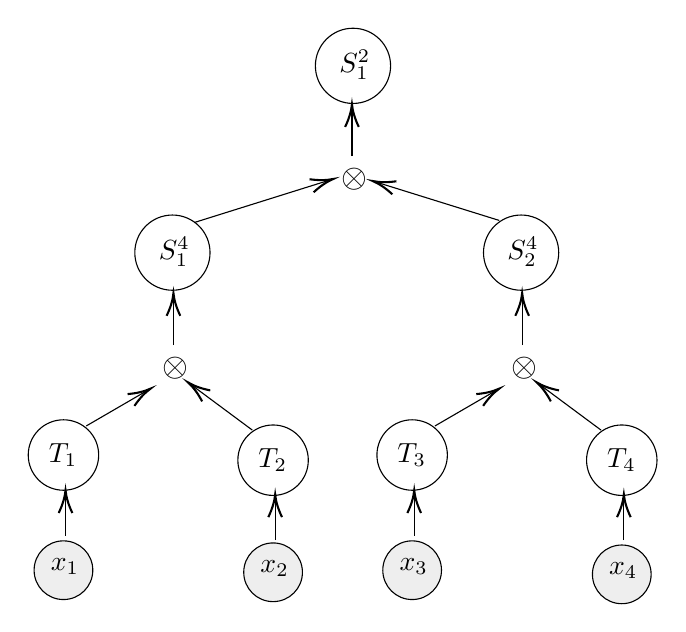
\begin{tikzpicture}[x=0.75pt,y=0.75pt,yscale=-1,xscale=1]

\draw    (148,113.5) -- (213.09,93.1) ;
\draw [shift={(215,92.5)}, rotate = 162.6] [color={rgb, 255:red, 0; green, 0; blue, 0 }  ][line width=0.75]    (10.93,-3.29) .. controls (6.95,-1.4) and (3.31,-0.3) .. (0,0) .. controls (3.31,0.3) and (6.95,1.4) .. (10.93,3.29)   ;
\draw    (295,112.5) -- (235.91,94.09) ;
\draw [shift={(234,93.5)}, rotate = 17.3] [color={rgb, 255:red, 0; green, 0; blue, 0 }  ][line width=0.75]    (10.93,-3.29) .. controls (6.95,-1.4) and (3.31,-0.3) .. (0,0) .. controls (3.31,0.3) and (6.95,1.4) .. (10.93,3.29)   ;
\draw    (176,213.5) -- (146.61,191.69) ;
\draw [shift={(145,190.5)}, rotate = 36.57] [color={rgb, 255:red, 0; green, 0; blue, 0 }  ][line width=0.75]    (10.93,-3.29) .. controls (6.95,-1.4) and (3.31,-0.3) .. (0,0) .. controls (3.31,0.3) and (6.95,1.4) .. (10.93,3.29)   ;
\draw    (96,211.5) -- (125.27,194.5) ;
\draw [shift={(127,193.5)}, rotate = 149.86] [color={rgb, 255:red, 0; green, 0; blue, 0 }  ][line width=0.75]    (10.93,-3.29) .. controls (6.95,-1.4) and (3.31,-0.3) .. (0,0) .. controls (3.31,0.3) and (6.95,1.4) .. (10.93,3.29)   ;
\draw    (138,172.5) -- (138,149.5) ;
\draw [shift={(138,147.5)}, rotate = 90] [color={rgb, 255:red, 0; green, 0; blue, 0 }  ][line width=0.75]    (10.93,-3.29) .. controls (6.95,-1.4) and (3.31,-0.3) .. (0,0) .. controls (3.31,0.3) and (6.95,1.4) .. (10.93,3.29)   ;
\draw    (86,264.5) -- (86,244.5) ;
\draw [shift={(86,242.5)}, rotate = 90] [color={rgb, 255:red, 0; green, 0; blue, 0 }  ][line width=0.75]    (10.93,-3.29) .. controls (6.95,-1.4) and (3.31,-0.3) .. (0,0) .. controls (3.31,0.3) and (6.95,1.4) .. (10.93,3.29)   ;
\draw    (187,266.5) -- (187,246.5) ;
\draw [shift={(187,244.5)}, rotate = 90] [color={rgb, 255:red, 0; green, 0; blue, 0 }  ][line width=0.75]    (10.93,-3.29) .. controls (6.95,-1.4) and (3.31,-0.3) .. (0,0) .. controls (3.31,0.3) and (6.95,1.4) .. (10.93,3.29)   ;
\draw    (344,213.5) -- (314.61,191.69) ;
\draw [shift={(313,190.5)}, rotate = 36.57] [color={rgb, 255:red, 0; green, 0; blue, 0 }  ][line width=0.75]    (10.93,-3.29) .. controls (6.95,-1.4) and (3.31,-0.3) .. (0,0) .. controls (3.31,0.3) and (6.95,1.4) .. (10.93,3.29)   ;
\draw    (264,211.5) -- (293.27,194.5) ;
\draw [shift={(295,193.5)}, rotate = 149.86] [color={rgb, 255:red, 0; green, 0; blue, 0 }  ][line width=0.75]    (10.93,-3.29) .. controls (6.95,-1.4) and (3.31,-0.3) .. (0,0) .. controls (3.31,0.3) and (6.95,1.4) .. (10.93,3.29)   ;
\draw    (306,172.5) -- (306,149.5) ;
\draw [shift={(306,147.5)}, rotate = 90] [color={rgb, 255:red, 0; green, 0; blue, 0 }  ][line width=0.75]    (10.93,-3.29) .. controls (6.95,-1.4) and (3.31,-0.3) .. (0,0) .. controls (3.31,0.3) and (6.95,1.4) .. (10.93,3.29)   ;
\draw    (254,264.5) -- (254,244.5) ;
\draw [shift={(254,242.5)}, rotate = 90] [color={rgb, 255:red, 0; green, 0; blue, 0 }  ][line width=0.75]    (10.93,-3.29) .. controls (6.95,-1.4) and (3.31,-0.3) .. (0,0) .. controls (3.31,0.3) and (6.95,1.4) .. (10.93,3.29)   ;
\draw    (355,266.5) -- (355,246.5) ;
\draw [shift={(355,244.5)}, rotate = 90] [color={rgb, 255:red, 0; green, 0; blue, 0 }  ][line width=0.75]    (10.93,-3.29) .. controls (6.95,-1.4) and (3.31,-0.3) .. (0,0) .. controls (3.31,0.3) and (6.95,1.4) .. (10.93,3.29)   ;
\draw    (224,81.5) -- (224,58.5) ;
\draw [shift={(224,56.5)}, rotate = 90] [color={rgb, 255:red, 0; green, 0; blue, 0 }  ][line width=0.75]    (10.93,-3.29) .. controls (6.95,-1.4) and (3.31,-0.3) .. (0,0) .. controls (3.31,0.3) and (6.95,1.4) .. (10.93,3.29)   ;

\draw    (137.5, 128) circle [x radius= 18.12, y radius= 18.12]   ;
\draw (128,117.4) node [anchor=north west][inner sep=2pt]    {$S_{1}^{4}$};
\draw    (224.5, 38) circle [x radius= 18.12, y radius= 18.12]   ;
\draw (215,27.4) node [anchor=north west][inner sep=2pt]    {$S_{1}^{2}$};
\draw    (186, 228) circle [x radius= 16.97, y radius= 16.97]   ;
\draw (176,219.4) node [anchor=north west][inner sep=2pt]    {$T_{2}$};
\draw (126,171.4) node [anchor=north west][inner sep=5pt]  [font=\large]  {$\otimes $};
\draw    (85, 225.5) circle [x radius= 16.97, y radius= 16.97]   ;
\draw (75,216.9) node [anchor=north west][inner sep=2pt]    {$T_{1}$};
\draw  [fill={rgb, 255:red, 238; green, 238; blue, 238 }  ,fill opacity=1 ]  (85, 281) circle [x radius= 14.14, y radius= 14.14]   ;
\draw (76,272.4) node [anchor=north west][inner sep=2pt]    {$x_{1}$};
\draw  [fill={rgb, 255:red, 238; green, 238; blue, 238 }  ,fill opacity=1 ]  (186, 282) circle [x radius= 14.14, y radius= 14.14]   ;
\draw (177,273.4) node [anchor=north west][inner sep=2pt]    {$x_{2}$};
\draw    (305.5, 128) circle [x radius= 18.12, y radius= 18.12]   ;
\draw (296,117.4) node [anchor=north west][inner sep=2pt]    {$S_{2}^{4}$};
\draw    (354, 228) circle [x radius= 16.97, y radius= 16.97]   ;
\draw (344,219.4) node [anchor=north west][inner sep=2pt]    {$T_{4}$};
\draw (294,171.4) node [anchor=north west][inner sep=5pt]  [font=\large]  {$\otimes $};
\draw    (253, 225.5) circle [x radius= 16.97, y radius= 16.97]   ;
\draw (243,216.9) node [anchor=north west][inner sep=2pt]    {$T_{3}$};
\draw  [fill={rgb, 255:red, 238; green, 238; blue, 238 }  ,fill opacity=1 ]  (253, 281) circle [x radius= 14.14, y radius= 14.14]   ;
\draw (244,272.4) node [anchor=north west][inner sep=2pt]    {$x_{3}$};
\draw  [fill={rgb, 255:red, 238; green, 238; blue, 238 }  ,fill opacity=1 ]  (354, 283) circle [x radius= 14.14, y radius= 14.14]   ;
\draw (345,274.4) node [anchor=north west][inner sep=2pt]    {$x_{4}$};
\draw (212,80.4) node [anchor=north west][inner sep=5pt]  [font=\large]  {$\otimes $};
\end{tikzpicture}
}
    \caption{Schematic view of the computational tree for \textsc{TreeSketch} for a tensor product of four vectors $x_1\otimes\dots\otimes x_4$.}
    \label{fig:treesketch}
\end{center}
\end{figure}

\section{Proofs}\label{proofs in appendix}

\subsection{Proof of Theorem \ref{thm:general-minmax-rf}}\label{apdx:minmax-rf-proof}

    For simplicity, we drop the subscripts $h,\Xi$ from probabilities and expectations. To show that the random features are unbiased, we re-write the expectation:
    \eq{
    &\mathbb{E}\left[ \phi_{\Xi,h}(x)\cdot \phi_{\Xi,h}(x')\right]  & \\
        &= \Pr(h(x)=h(x')) \mathbb{E} \left[ \Xi_{h(x)}\Xi_{h(x')} | h(x)=h(x')\right]  \nonumber & \\
           &\quad+ \Pr(h(x)\neq h(x')) \mathbb{E} \left[ \Xi_{h(x)}\Xi_{h(x')} | h(x)\neq h(x')\right] &\\
        &= \Pr(h(x)=h(x')) \mathbb{E} \left[ \Xi_{h(x)}^2 \right] &\text{(}\Xi_{h(x)}=\Xi_{h(x')}\text{)} \nonumber \\
        &\quad+ \Pr(h(x)\neq h(x')) \mathbb{E} \left[\Xi_{h(x)}\right] \mathbb{E} \left[\Xi_{h(x')}\right] & (\Xi_{h(x)},\Xi_{h(x')}\text{ independent)} \\
        &= 1\cdot \Pr(h(x)=h(x')) + 0\cdot \Pr(h(x)\neq h(x')) &\text{(assumed moments of }\xi) \\
        &= T_{MM}(x,x')& \text{($h(x)$ is an unbiased hash for $T_{MM}$)}
    }

    Because in general $\mathbb{V}[X]=\mathbb{E}[X^2]-\mathbb{E}[X]^2$,
    and we have $\mathbb{E}\left[ \phi_{\Xi,h}(x)\cdot \phi_{\Xi,h}(x')\right]=T_{MM}(x,x')$,
    we only need to compute
    $\mathbb{E}\left[ \left(\phi_{\Xi,h}(x)\cdot \phi_{\Xi,h}(x')\right)^2\right]$.
    This can be done using a similar decomposition:
    \eq{
        \mathbb{E}\left[ \left(\phi_{\Xi,h}(x)\cdot \phi_{\Xi,h}(x')\right)^2\right]&= \Pr(h(x)=h(x')) \mathbb{E}\left[ \left(\phi_{\Xi,h}(x)\cdot \phi_{\Xi,h}(x')\right)^2|h(x)=h(x')\right] \nonumber \\
        &\quad + \Pr(h(x)\neq h(x')) \mathbb{E}\left[ \left(\phi_{\Xi,h}(x)\cdot \phi_{\Xi,h}(x')\right)^2|h(x)\neq h(x')\right] \\
        &= T_{MM}(x,x') \mathbb{E}\left[ \Xi_{h(x)}^4 \right] \nonumber \\
        &\quad + \left(1-T_{MM}(x,x')\right) \mathbb{E}\left[ \Xi_{h(x)}^2 \right] \mathbb{E}\left[ \Xi_{h(x')}^2 \right] \\
        &= T_{MM}(x,x') \mathbb{E}\left[ \Xi_{h(x)}^4 \right] + \left(1-T_{MM}(x,x')\right) 
    }
    Here, the last step follows from the moments of $\Xi$ which were fixed by assumption.
    Subtracting $T_{MM}(x,x')^2$ from the above yields the expression for the variance.

By Jensen's inequality, $\E[\xi^4]\geq \E[\xi^2]^2$, and $\E[\xi^2]=1$ by assumption, so $\E[\xi^4]\geq1$.
    Substituting $\E[\xi^4]=1$ into the equation for $\mathbb{V}(\phi_{\Xi,h}(x)\cdot \phi_{\Xi,h}(x'))$ gives the lower bound and completes the proof.

\subsection{Proof of Theorem \ref{thm:tdp-is-pd} and Corollary \ref{thm:tdp-is-metric}}\label{apdx:tdp-is-pd-proof}

Take any pair of inputs $x,y\neq 0$ in $\R^d$. By the Cauchy--Schwarz inequality, we have
\numeq{ \label{eq:term-bound}
\Bigg| \frac{x\cdot y}{|x|^2 + |y|^2} \Bigg|\leq \frac{|x||y|}{|x|^2 + |y|^2} \leq \left(|x|/|y| + \frac{1}{|x|/|y|} \right)^{-1} \leq \frac{1}{2}.
}
Now, we can write the function $T_{DP}$ as
\begin{align}
    T_{DP}(x,y) = \frac{x\cdot y}{|x|^2 + |y|^2 - x\cdot y} &= \frac{\frac{x\cdot y}{|x|^2 + |y|^2}}{1 - \frac{x\cdot y}{|x|^2 + |y|^2}} \label{eqn:power-series1} \\
    &= \frac{x\cdot y}{|x|^2 + |y|^2}\left(\frac{1}{1 - \frac{x\cdot y}{|x|^2 + |y|^2}}\right) \label{eqn:power-series2} \\
    &= \frac{x\cdot y}{|x|^2 + |y|^2} \sum_{r=0}^\infty \left(\frac{x\cdot y}{|x|^2 + |y|^2}\right)^r \label{eqn:power-series3} \\
    &= \sum_{r=1}^\infty \left(\frac{x\cdot y}{|x|^2 + |y|^2}\right)^r \label{eqn:power-series},
\end{align}
where in the identity (\ref{eqn:power-series3}) we use the bound in (\ref{eq:term-bound}) to assert that the series is bounded by $2^{-r}$ and thus absolutely convergent.

Furthermore, because $(x,y)\mapsto x\cdot y$ is a positive definite kernel, and so is
$$(x,y)\mapsto \frac{1}{|x|^2+|y|^2 } = \int_{0}^\infty  e^{-(|x|^2+|y|^2)t}  dt,$$
each summand in the power series is positive definite because it is a product of positive definite kernels.
Hence, as sums and limits of positive definite kernels are positive definite, and the power series is convergent, $T_{DP}$ is positive definite in the space $\R^d\setminus \{0\}$. The extension to include the vector $0\in\R^d$ is straightforward, as any Gram matrix including this vector is block diagonal. We conclude that $T_{DP}$ is a positive definite kernel in $\R^d$. 

To prove Corollary \ref{thm:tdp-is-metric}, note that by the Moore--Aronszajn theorem, there exists an RKHS of functions $(\mathcal H, \langle\cdot\rangle_\mathcal{H})$ on $\R^d$ with reproducing kernel $T_{DP}$, such that for any $x,y\in\R^d$, $\langle T_{DP}(x,\cdot), T_{DP}(y,\cdot) \rangle_\mathcal{H} = T_{DP}(x,y)$. Then, observe that 
\eq{
\|T_{DP}(x,\cdot)-T_{DP}(y,\cdot)\|_\mathcal{H}^2
&= \langle T_{DP}(x,\cdot)- T_{DP}(y,\cdot),T_{DP}(x,\cdot)- T_{DP}(y,\cdot) \rangle_\mathcal{H} \\
&= \langle T_{DP}(x,\cdot),T_{DP}(x,\cdot) \rangle_\mathcal{H} 
+ \langle T_{DP}(y,\cdot), T_{DP}(y,\cdot) \rangle_\mathcal{H} \\
& ~~~~~- 2 \langle T_{DP}(x,\cdot), T_{DP}(y,\cdot) \rangle_\mathcal{H} \\
& = 2 - 2T_{DP}(x,y),
}
where in the final identity, we use the fact that $T_{DP}(x,x)=1$ for all $x\in\R^d$. Dividing by 2 and taking square roots on both sides, we obtain
\eq{
\Big\|\frac{1}{2}T_{DP}(x,\cdot)-\frac{1}{2}T_{DP}(y,\cdot)\Big\|_\mathcal{H} = \sqrt{1-T_{DP}(x,y)},
}
where the RKHS norm on the left is clearly a distance metric. 

\subsection{Sketch of the kernel $(|x|^2 + |x'|^2)^{-r}$}
\label{apdx:prefactor-sketch}

This section develops a sketch for the positive definite kernel $(x,x')\mapsto (|x|^2 + |x'|^2)^{-r}$ defined in Section \ref{sec:tdp-rf}, and gives proofs for Lemmas \ref{QMC error} and \ref{QMC estimator unbiased}.

As the kernel is a function of $|x|^2$ and $|x'|^2$, we can deal, without loss of generality, with the one-dimensional case. We begin by observing that for any $a,b>0$,
\numeq{
\left(\frac{1}{a+b}\right)^r 
&= \int_0^\infty e^{(1/2-a)t}e^{(1/2-b)t} \frac{t^{r-1} e^{-t}}{\Gamma(r)}dt \nonumber \\
&= \int_0^\infty e^{(1/2-a)t}e^{(1/2-b)t}c^{-r}e^{(c-1)t} \frac{c^r t^{r-1} e^{-ct}}{\Gamma(r)}dt \nonumber \\
&= \int_0^\infty e^{(1/2-a)t}e^{(1/2-b)t}\frac{c^{-s}e^{(c-1)t}t^{r-s}\Gamma(s)}{\Gamma(r)} \frac{c^s t^{s-1} e^{-ct}}{\Gamma(s)}dt. \label{1}
}
Defining the function
\eq{
\varphi_Z(a) = e^{(1/2-a)Z} Z^{(r-s)/2}\left(\frac{c^{-s}e^{(c-1)Z}\Gamma(s)}{\Gamma(r)} \right)^{1/2}
}
and letting $Z\sim\text{Gamma}(s,c)$, we recognise the right hand side of (\ref{1}) as the expectation of $\varphi_Z(a)\varphi_Z(b)$. Hence, 
\eq{
\left(\frac{1}{a+b}\right)^r = \E(\varphi_Z(a)\varphi_Z(b)).
}
It is possible to sketch $a$ with a vector $\varphi(a) = \frac{1}{\sqrt{M}}(\varphi_{Z_1}(a),\dots,\varphi_{Z_M}(a))$ where $Z_1,\dots,Z_M$ are independent copies of $Z$. This makes the kernel approximation $\varphi(a)\cdot \varphi(b)$ a Monte Carlo estimator of the expectation, with error decreasing with the dimension $M$ of the sketch at the standard rate $O(M^{-1/2})$. 

However, we shall instead consider a Quasi-Monte Carlo (QMC) estimator with an error decreasing at the faster rate $O(M^{-1})$. We will derive a uniform error bound, and then tune the parameters $(c,s)$ so as to minimise it. 

Let $\gamma_{s,c}$ be the inverse cumulative distribution function of a Gamma$(s,c)$ random variable. With a change of variables, we can write the integral (\ref{1}) as 
\numeq{ \label{eq:ch-of-variables}
\left(\frac{1}{a+b}\right)^r 
& = \frac{c^{-s}\Gamma(s)}{\Gamma(r)} \int_0^1 e^{-(a+b-c)\gamma_{s,c}(u)} (\gamma_{s,c}(u))^{r-s}  du.
}
Fix $n>0$, $u\in[0,1]$, and let $u_i = (u + i/M)- \lfloor u + i/M \rfloor $ for $i=1,\dots,M$. We can now define features $\phi_{u,r}(a)\in \R^M$, as in Section \ref{sec:tdp-rf}:
\eq{
\phi_{u,r,i}(a) =\frac{1}{\sqrt M}\sqrt{\frac{c^{-s}\Gamma(s)}{\Gamma(r)} } e^{-(a-c/2)\gamma_{s,c}(u_i) }(\gamma_{s,c}(u_i))^{(r-s)/2}.
}
A QMC estimator for $(a+b)^{-r}$ is given by the dot product $\phi_u(a)^T \phi_u(b)$. At this stage, we can prove Lemma \ref{QMC estimator unbiased}, which is restated here for convenience.

\begin{lemma*}[Main text \ref{QMC estimator unbiased}]
If $u$ is random and $\mathcal U(0,1)$, then for all $a,b>0$,
\eq{
\left(\frac{1}{a+b}\right)^r = \E(\phi_{u,r}(a)\cdot \phi_{u,r}(b)).
}
\end{lemma*}
\begin{proof}
By linearity of expectation,
\eq{
\E(\phi_{u,r}(a)\cdot \phi_{u,r}(b)) = \frac{1}{M}\sum_{i=1}^M \E\left[\frac{c^{-s}\Gamma(s)}{\Gamma(r)}  e^{-(a+b-c)\gamma_{s,c}(u_i) }(\gamma_{s,c}(u_i))^{r-s} \right].
}
Observing that each $u_i\sim\mathcal U(0,1)$, the result follows by Eq.\ (\ref{eq:ch-of-variables}).
\end{proof}

In the following lemma, we establish a basic Quasi-Monte Carlo error bound.

\begin{lemma}\label{QMC basic lemma} 
For any $u\in[0,1]$, $c\leq (a+b)$, $0<s \le r $,
\eq{
\Big| \frac{1}{(a+b)^r} - \phi_{u,r}(a) \cdot \phi_{u,r}(b) \Big| \leq \frac{2}{M} \frac{c^{-s}\Gamma(s)}{\Gamma(r)} \left(\frac{r-s}{e(a+b-c)}\right)^{r-s}.
}
\end{lemma}

\begin{proof}
Consider the QMC approximation of an integral $\int_0^1 f(x)dx$ for a function $f$ of bounded variation, using a regular net of $n$ points. It is well known that the error of this approximation is bounded above by $V(f)/n$ where $V$ is the total variation norm. Hence, 
\eq{
\Big| \frac{1}{(a+b)^r} - \phi_{u,r}(a)\cdot \phi_{u,r}(b) \Big| \leq \frac{1}{n} \frac{c^{-s}\Gamma(s)}{\Gamma(r)} V(f)
}
for $f(u)= e^{-(a+b-c)\gamma_{s,c}(u)} (\gamma_{s,c}(u))^{r-s}$ on $0\leq u\leq 1$. As $\gamma_{s,c}$ is monotone increasing, $f$ is unimodal tending to $0$ as $u\to 0$ and $u\to 1$. Thus $V(f)=2\max_{0\le u\le 1} f(u)$.
The maximum of $f$ is attained where $\gamma_{s,c}(u)= (r-s)/(a+b-c)$, hence 
\eq{
V(f) = 2\left(\frac{r-s}{e(a+b-c)}\right)^{r-s}. & \qedhere
}
\end{proof}

We are interested in sketching $( | x_i | ^2+ | x_j | ^2)^{-r}$ for every pair of inputs $x_i, x_j$ in a dataset $\{x_1,\dots,x_n\}$. The previous lemma can be used to choose values $c$ and $s\le r$ which minimise the relative error
\eq{
E_{i,j} = \frac{   \phi_{u,r}(  x_i )\cdot \phi_{u,r}( x_j ) - (| x_i | ^2+ | x_j | ^2)^{-r} }{( | x_i | ^2+ | x_j | ^2)^{-r}} .
}

The kernel $k(x,y)$ is invariant to scaling $x$ and $y$, \emph{i.e.}, $k(x,y)=k(\ell x,\ell y)$ for all $\ell>0$. Thus, if we are interested in approximating the Gram matrix for $\{x_1,\dots,x_n\}$, we may assume without loss of generality that $\max_i  | x_i | ^2 = 1$ and let $\zeta = \min_i  | x_i | ^2$. Here, $\zeta$ will act as a condition number for the dataset, which will determine the error of the random feature approximation.

By Lemma \ref{QMC basic lemma}, we have
\eq{
|E_{i,j} |
&\leq ( | x_i | ^2+ | x_j | ^2)^r \frac{2}{M} \frac{c^{-s}\Gamma(s)}{\Gamma(r)} \left(\frac{r-s}{e( | x_i | ^2+ | x_j | ^2-c)}\right)^{r-s} \\
&= ( | x_i | ^2+ | x_j | ^2)^r \frac{2}{M} \frac{c^{-s}\Gamma(s)(r-s)^{r-s}}{\Gamma(r)e^{(r-s)}} \left(\frac{1}{ | x_i | ^2+ | x_j | ^2-c}\right)^{r-s} \\
&= \frac{2}{M} \frac{\Gamma(s)(r-s)^{r-s}}{\Gamma(r)e^{(r-s)}} \left(1-\frac{c}{ | x_i | ^2+ | x_j | ^2}\right)^{s-r} \left(\frac{c}{ | x_i | ^2+ | x_j | ^2}\right)^{-s} .
} 
The last two factors are log-convex in $c/( | x_i | ^2+ | x_j | ^2)>0$. Hence, for a fixed $c$, the product
$$\left(1-\frac{c}{ | x_i | ^2+ | x_j | ^2}\right)^{s-r} \left(\frac{c}{ | x_i | ^2+ | x_j | ^2}\right)^{-s} $$
 is maximised at either $ | x_i | ^2+ | x_j | ^2=2$ or $ | x_i | ^2+ | x_j | ^2=2\zeta$. Therefore,
\eq{
|E_{i,j}|
&\leq \frac{2}{M} \frac{\Gamma(s)(r-s)^{r-s}}{\Gamma(r)e^{(r-s)}} \left[\left(1-\frac{c}{2}\right)^{s-r} \left(\frac{c}{2}\right)^{-s} \vee \left(1-\frac{c}{2\zeta}\right)^{s-r} \left(\frac{c}{2\zeta}\right)^{-s}\right].
} 
Using again the log-convexity of $y\mapsto (1-y)^{s-r} y^{-s}$, we find that 
$$\left(1-\frac{c}{2}\right)^{s-r} \left(\frac{c}{2}\right)^{-s} $$
is minimised as a function of $c$ at $c_1 = 2s/r$. And
$$\left(1-\frac{c}{2\zeta}\right)^{s-r} \left(\frac{c}{2\zeta}\right)^{-s}$$
is minimised at $c_2 = 2\zeta s/r$. Recall that Lemma \ref{QMC basic lemma} requires $0\le c\leq  | x_i | ^2+ | x_j | ^2$ for all $i,j$ or $0\le c\leq 2\zeta$, which is satisfied by $c_2$ when $s\le r$, but not necessarily by $c_1$. Thus, it is reasonable to set $c=c_2$, which leads to
\eq{
|E_{i,j}| 
&\leq \frac{2}{M} \frac{\Gamma(s)(r-s)^{r-s}}{\Gamma(r)e^{(r-s)}} \left[\left(1-\frac{\zeta s}{r}\right)^{s-r} \left(\frac{\zeta s}{r}\right)^{-s} \vee \left(1- \frac{s}{r}\right)^{s-r} \left( \frac{s}{r}\right)^{-s}\right] \\
&\leq \frac{2}{M} \frac{\Gamma(s)(r-s)^{r-s}r^{r}s^{-s}}{\Gamma(r)e^{(r-s)}} \left[\left(r-\zeta s\right)^{s-r} \zeta^{-s} \vee \left(r- s\right)^{s-r} \right] \\
&\leq \frac{2}{M} \frac{\Gamma(s)(s/e)^{-s}}{\Gamma(r)(r/e)^{-r}} \left[\left(\frac{r-\zeta s}{r-s}\right)^{s-r} \zeta^{-s} \vee 1 \right] .
} 
When $\zeta=1$ (all inputs $x_i$ have the same norm), setting $s=r$ leads to an  error bound of $4/n$. However, small values of $\zeta$ can make the upper bound blow up unless we tune $s$ suitably. For a given value of $\zeta$, this upper bound could be maximised numerically over $0<s\le r$. However, setting $s = r\zeta$, we obtain
\eq{
|E_{i,j}|
&\leq \frac{2}{M} \frac{\Gamma(r\zeta)(r\zeta /e)^{-r\zeta}}{\Gamma(r)(r/e)^{-r}} \left[\left(\frac{1-\zeta^2}{1-\zeta}\right)^{r(\zeta-1)} \zeta^{-r\zeta} \vee 1 \right]  \\
&\leq \frac{2}{M} \frac{\Gamma(r\zeta)\zeta^{-r\zeta}}{\Gamma(r)} (r/e)^{r(\zeta-1)}\left[\left(\left(\frac{1-\zeta^2}{1-\zeta}\right)^{\zeta-1} \zeta^{-\zeta}\right)^r \vee 1 \right] \\
&\leq \frac{2}{M} \frac{\Gamma(r\zeta)\zeta^{-r\zeta}}{\Gamma(r)} (r/e)^{r(\zeta-1)} \rho^r
} 
where $\rho\approx 1.2$ is defined by 
$$\rho := \max_{0\leq \zeta\leq 1}~\left(\frac{1-\zeta^2}{1-\zeta}\right)^{\zeta-1} \zeta^{-\zeta}.$$
This proves the first inequality in Lemma \ref{QMC error}. 

To conclude the proof of Lemma \ref{QMC error}, we study the behaviour of the upper bound as it diverges when $\zeta\to 0$. Using the asymptotic $\Gamma(x)\sim 1/x$ as $x\to0$, we have
\eq{
\frac{2}{M} \frac{\Gamma(r\zeta)\zeta^{-r\zeta}}{\Gamma(r)} (r/e)^{r(\zeta-1)} \rho^r \sim (M\zeta)^{-1} \frac{2(r/e)^{-r} \rho^r}{r\Gamma(r)} 
}
where $\frac{2(r/e)^{-r} \rho^r}{r\Gamma(r)}$ is bounded for $r\ge 1$. Therefore, the upper bound is $O(M^{-1}\zeta^{-1})$. 

\subsection{Proof of Theorem \ref{error bound theorem}}
\label{apdx:proof-of-error-bound}

We begin by defining the stable rank, a common notion of effective dimension for a data matrix $A\in\R^{d\times n}$ or its associated Gram matrix $A^TA$.

\begin{definition}
The \emph{stable rank} $\text{sr}(A)$ of a data matrix $A\in\R^{d\times n}$ is given by
\eq{
\text{sr}(A) = \frac{\|A\|_F^2}{\|A\|^2_\text{op}}.
}
For a positive semi-definite matrix $K\in\R^{n\times n}$, define $\tilde{\text{sr}}(K) = \Tr(K)/\|K\|_\text{op}$.
\end{definition}

The stable rank of $A$ is upper bounded by the rank, but it is insensitive to small singular values, so it can be much smaller than $\min(n,d)$. Note that $\text{sr}(A) = \tilde{\text{sr}}(A^TA)$. The function $\tilde{\text{sr}}(K)$ extends the concept of stable rank to a general kernel matrix $K$. 

We now re-state \cref{error bound theorem} for convenience, and provide a proof:

\begin{theorem*} 
For any $n\ge 1$, let $x_1,\dots,x_n\in\R^d$ be a set of inputs with $\frac{\min_i |x_i|^2}{\max_i |x_i|^2} \geq \zeta$. Let $K$ be the matrix with entries $K_{i,j} = T_\text{DP}(x_i,x_j)$. For all $\varepsilon>0$, there exists an oblivious sketch $\Phi:\R^d \to \R^m$ with $m=\tilde\Omega(\tilde{\text{sr}}(K) /\varepsilon^{2})$, such that 
\eq{
\Pr_{\Phi}\Big(\|\widehat K-K\|_\text{op} \ge\varepsilon \|K\|_\text{op}) \leq \frac{1}{\text{poly}(n)}
}
where $\widehat K_{i,j} = \Phi(x_i)\cdot \Phi(x_j)$. Furthermore, the sketch can be computed in time $\tilde O(\tilde{\text{sr}}(K)n\varepsilon^{-2}+\text{nnz}(X)\varepsilon^{-2}+n\zeta^{-1}\varepsilon^{-3})$.
\end{theorem*}

For each $r\in[R]$, define matrices $K^r$, $\tilde K^r$, and $\widehat K^r$ in $\R^{n\times n}$ by
\eq{
K^r_{i,j} &= \left(\frac{x_i\cdot x_j}{|x_i|^2+|x_j|^2}\right)^r, \\
\tilde K^r_{i,j} & = (x_i^{\otimes r} \otimes \phi_{u,r}(x_i))\cdot (x_i^{\otimes r} \otimes \phi_{u,r}(x_i)), \\
\widehat K^r_{i,j} &= \Phi_r(x_i)\cdot \Phi_r(x_j).
} 
Then, by the triangle inequality, we have
\numeq{
\|\widehat K - K\|_\text{op} 
&\leq \sum_{r=1}^R \|\widehat K^r - \tilde K^r \|_\text{op} + \sum_{r=1}^R \| \tilde K^r-K^r \|_\text{op}+ \left\|\sum_{r=1}^R K^r - K\right\|_\text{op} \nonumber \\
&\leq \sum_{r=1}^R \|\widehat K^r - \tilde K^r \|_\text{op} + \sum_{r=1}^R \| \tilde K^r-K^r \|_\text{op}+ \sum_{r=R+1}^\infty \|K^r \|_\text{op}. \label{terms}
}
We shall find high-probability bounds for each of the terms on the right in turn. For the last term, we can choose $R=C \log(\tilde{\text{sr}}(K) \varepsilon^{-1})$ with $C$ large enough, and apply the following upper bound
\numeq{ 
\sum_{r=R+1}^\infty \|K^r \|_\text{op} 
&\leq \sum_{r=R+1}^\infty \|K^r \|_F \nonumber \\
&\leq \sum_{r=R+1} n \left(\max_{i,j\in[n]} \frac{|x_i\cdot x_j|^r}{(|x_i^2|+|x_j|^2)^r}\right)^{1/2} \nonumber \\
&\leq \sum_{r=R+1} n2^{-r/2} \nonumber \\
&\leq n2^{-(R-1)/2}  \leq \frac{n\varepsilon }{3\tilde{\text{sr}}(K)} \leq  \frac{\varepsilon \|K\|_\text{op}}{3}, \label{third term}
}
where the final inequality follows from the fact that $\tilde{\text{sr}}(K) = n/\|K\|_\text{op}$, as the kernel matrix $K$ has ones on the diagonal. 

The terms in the second sum of (\ref{terms}) may be written as
\eq{
\| \tilde K^r-K^r \|_\text{op} = \| \tilde E\odot K^r \|_\text{op}
}
where $\odot$ denotes the Hadamard product and $E$ is the error matrix defined in (\ref{error matrix}). Noting that $E$ is symmetric, we can apply Corollary 11 in \cite{ando1987singular} %
to assert that
\eq{
\| \tilde K^r-K^r \|_\text{op} \leq \max_i |E_{i,i}| \|K^r\|_\text{op}.
}
By the triangle inequality, for each $r\ge 1$, we have $\|K^r\|_\text{op}\leq \|K\|_\text{op}$. Hence, with the choice $M=\Omega(R \zeta^{-1}\varepsilon^{-1})$, and applying Lemma \ref{QMC error} we obtain
\numeq{ \label{second term}
\sum_{r=1}^R \| \tilde K^r-K^r \|_\text{op} \leq \frac{\varepsilon\|K\|_\text{op}}{3}.
}

Finally, we turn to the first term in (\ref{terms}). Let $A_r$ be a matrix with columns $x_i^{\otimes r} \otimes \phi_{u,r}(x_i)$ for $i=1,\dots,n$. We can rewrite the error in question
\eq{
\|\widehat K^r - \tilde K^r \|_\text{op} = \| (\Pi^{r+1} A_r )^T\Pi^{r+1} A_r -A_r^TA_r\|_\text{op}
}
In Lemma \ref{A norm bounds}, we establish that $\|A_r\|_F^2\leq (1+\varepsilon)\Tr(K)$ and $\|A_r\|^2_\text{op}\leq (1+\varepsilon)\|K\|_\text{op}$. Let $\delta = 1/\text{poly}(n)$ denote the error tolerance. Choose the dimension of the sketch $\Pi^{r+1}$ to be $m_r = \Omega\left(\frac{R^2 r^4 \tilde{\text{sr}}(K)}{\varepsilon^2}\log^3\left(\frac{n(d\vee M)}{\varepsilon \delta}\right)\right)$ and the sparsity parameter of \textsc{OSNAP} as $s=\frac{R^2 r^4}{\varepsilon^2}\log^3\left(\frac{n(d\vee M)}{\varepsilon \delta}\right)$. Then, Lemmata 32--34 in \cite{ahle2020oblivious} ensure that, 
\eq{
\Pr\left(\|\widehat K^r - \tilde K^r \|_\text{op} \geq \frac{\varepsilon\|K\|_\text{op}}{3R} \right) = \Pr\left(\| (\Pi^{r+1} A_r )^T\Pi^{r+1} A_r -A_r^TA_r\|_\text{op} \geq \frac{\varepsilon\|K\|_\text{op}}{3R} \right) \le \frac{1}{\text{poly}(n)}.
}
Taking a union bound, we obtain 
\numeq{ \label{first term}
\Pr\left(\sum_{r=1}^R\|\widehat K^r - \tilde K^r \|_\text{op} \ge \frac{\varepsilon\|K\|_\text{op}}{3} \right) \le \frac{1}{\text{poly}(n)}.
}
Finally, combining the bounds (\ref{first term}), (\ref{second term}), and (\ref{third term}), we obtain 
\eq{
\Pr\left (\|\widehat K - K\|_\text{op}  \ge \varepsilon\|K\|_\text{op}\right) \le \frac{1}{\text{poly}(n)}.
}

\paragraph{Dimension of the sketch $\Phi$:} The total dimension of the sketch is $m=m_1+\dots+m_R$, where $m_r =  \Omega\left(\frac{R^2 r^4 \tilde{\text{sr}}(K)}{\varepsilon^2}\log^3\left(\frac{n(d\vee M)}{\varepsilon \delta}\right)\right)$ with $R = C \log(\tilde{\text{sr}}(K) \varepsilon^{-1})$. Hence, ignoring poly-logarithmic factors, the sketch has dimension $m = \tilde \Omega(\tilde{\text{sr}}(K)/\varepsilon^2)$.

\paragraph{Runtime:} We first estimate the runtime of applying $\Phi_r$. Applying \textsc{OSNAP} with sparsity parameter $s$ to a vector $w\in\R^d$ takes $O(s\text{nnz}(w))$ time. Thus, applying $r$ independent  \textsc{OSNAP}  sketches to each $x_i$ for $i\in[n]$ takes $O(sr\text{nnz}(X))$ time. Applying \textsc{OSNAP} to $\phi_{u,r}(x_i)$ for $i\in[n]$ takes $O(nsM)$ time.  
Then, applying one \textsc{TensorSRHT} sketch takes $O(m_r\log m_r)$ time, and therefore applying all the necessary copies of $S_\text{base}$ requires $O(r m_r\log m_r)$. In total, the sketch $\Phi_r$ may be computed in $O(n r m_r\log m_r + s\text{nnz}(X) + nsM)$. Adding these runtimes over $r\in [R]$ gives us a total runtime which is $\tilde O(\tilde{\text{sr}}(K)n\varepsilon^{-2}+\text{nnz}(X)\varepsilon^{-2}+n\zeta^{-1}\varepsilon^{-3})$.\\

\begin{lemma}\label{A norm bounds}
For each $r=1,\dots, R$, we have $\|A_r\|_\text{op}^2\leq (1+\varepsilon)\|K\|_\text{op}$ and $\|A_r\|_F^2 \leq (1+\varepsilon)\Tr(K)$.
\end{lemma}

\begin{proof}
Note that $A_r^T A_r = \tilde K^r$. Hence, we aim to show that $\|\tilde K^r\|_\text{op}\leq (1+\varepsilon)\|K\|_\text{op}$, and that $\Tr(\tilde K^r) \leq(1+\varepsilon)\Tr(K)$. By the triangle inequality, 
\eq{
\|\tilde K^r\|_\text{op} \leq \|\tilde K^r\|_\text{op} + \|\tilde K^r - K^r\|_\text{op} \leq (1+\varepsilon)\|K^r\|_\text{op} \leq (1+\varepsilon)\|K\|_\text{op},
}
where the penultimate inequality was shown in the proof of Theorem \ref{error bound theorem}, and the final inequality is due to the fact that $K^r\preceq K$. 

Then, by linearity of the trace,
\numeq{
\Tr(\tilde K^r) = \Tr(K^r) + \Tr(\tilde K^r - K^r)  =\Tr(K^r) + \Tr(E\odot K^r). \label{trace bound}
}
And applying once more Corollary 11 of \cite{ando1987singular}, we have
\eq{
\Tr(E\odot K^r)  = \sum_{i=1}^n \sigma_i(E\odot K^r) \leq \max_{i\in[n]} |E_{i,i}| \sum_{i=1}^n \sigma_i(K^r) \leq \varepsilon \sum_{i=1}^n \sigma_i(K^r),
}
where $\sigma_i(\cdot)$ denotes the $i$th singular value. Using once more that $K^r\preceq K$ and hence $\sigma_i(K^r)\leq \sigma_i(K)$ for all $i\in[n]$, we obtain,
\eq{
\Tr(E\odot K^r) \leq \varepsilon \Tr(K).
}
Plugging this into (\ref{trace bound}) yields $\Tr(\tilde K^r) \leq(1+\varepsilon)\Tr(K)$.
\end{proof}

\section{Details of $T_{DP}$ sketch used in Section \ref{sec:experiments}}
\label{apdx:bias-correction}

Here, we describe several modifications of the sketch described in Section \ref{sec:tdp-rf} which were implemented in the experimental section. 

We begin by noting that when $x,x'\in\R_{\ge 0}^d$, $x\cdot x'\ge 0$, and therefore, the power series
\eq{
T_{DP}(x,x')=\sum_{r=1}^\infty (x\cdot x')^r(|x|^2+|x'|^2)^{-r}
}
is monotone. Therefore, if we use an unbiased sketch for the truncated series 
\eq{
\sum_{r=1}^R (x\cdot x')^r(|x|^2+|x'|^2)^{-r}
}
as the one constructed in Section \ref{sec:tdp-rf}, the final sketch will be biased \emph{downward}:
\eq{
\E(\Phi(x)\cdot\Phi(x'))< T_{DP}(x,x')
}
for all $x,x'\in\R_{\ge 0}^d$. Below we introduce two strategies to remedy this issue.

\subsection{Bias correction strategy 1: normalize the features}

Empirically, we observe that the highest bias occurs in the diagonal elements of the kernel matrix. As the kernel satisfies $T_{DP}(x,x)=1$ for all $x\in\R^d$, one possible correction is to \emph{normalize} the sketch to obtain
\eq{
\tilde \Phi(x) = \frac{\Phi(x)}{|\Phi(x)|}.
}
This remains an oblivious sketch, and ensures that the diagonal of the kernel matrix is estimated exactly, at the expense of possibly introducing some bias in off-diagonal elements of $K$.

\subsection{Bias correction strategy 2: sketch the residual}

To simplify the algebra,
let $t_{x,y}=\frac{x\cdot y}{|x|^2 + |y|^2}$.
The power series for $T_{DP}$ can then be re-written as:
\begin{align}
    T_{DP}(x,y) &= \sum_{r=1}^\infty \left(t_{x,y}\right)^r \nonumber\\
    &= \sum_{r=1}^{R} \left(t_{x,y}\right)^r + \left(t_{x,y}\right)^{R+1} + \sum_{r=R+2}^{\infty} \left(t_{x,y}\right)^r \nonumber\\
    &= \sum_{r=1}^{R} \left(t_{x,y}\right)^r + \left(t_{x,y}\right)^{R+1} + \left(t_{x,y}\right)^{R+1}\sum_{r=1}^{\infty} \left(t_{x,y}\right)^r \nonumber\\
    &= \underbrace{\sum_{r=1}^{R} \left(t_{x,y}\right)^r}_{k^{R}} + \underbrace{\left(t_{x,y}\right)^{R+1} \left(1 + T_{DP}(x,y)\right)}_{\text{truncation error}}
\end{align}
Critically, the truncation error can be written in terms of the kernel value itself, without any infinite sums.
This enables a simple procedure to generate random features for \emph{both} the truncated
power series and the remainder:
\begin{enumerate}
    \item Compute and store $\Phi(x)$ 
        as random features for the truncated kernel $k^{R}$.
    \item  Concatenate a single 1 onto $\Phi(x)$
        to produce features $\Phi_{+1}(x) = (1,\Phi(x))$ which approximate the kernel $1+k^{R}$
        using only a single extra dimension.
        Treat this as approximate random features for the kernel $1+k$.
    \item Compute random features $\Phi_{r+1}(x)$ for $t_{x,y}^{R+1}$.
    \item Apply \textsc{TensorSRHT} to the tensor product $\Phi_{r+1}(x)\otimes \Phi_{+1}(x)$ to obtain $\Delta(x)$,
        which approximates random features of the truncation error 
        $t_{x,y}^{R+1}(1+T_{DP}(x,y))$.
    \item Concatenate the random features $\Phi(x)$ and $\Delta(x)$, to obtain bias corrected random features $\Phi_\text{bc}(x)=\Phi\oplus \Delta(x)$.
\end{enumerate}

Overall, these random features are essentially a concatenation of
the random features for the truncated power series
with an additional random feature estimate of the truncation error,
which is formed using both the random features for the first $R$ terms
and the random features for the $(R+1)$th term.
A nice property of the procedure above is that it \emph{re-uses}
the random features $\Phi(x)$ to estimate the error.

\section{Experimental details and Additional Results}\label{appendix experimental details}

\subsection{Additional details for section~\ref{sec:expt-rf-on-real-data}}\label{apdx:rf-real-data-details}

\paragraph{Dataset}
Figure~\ref{fig:rf-experiment-dataset-summary} shows the number of atoms and the fingerprint norms
for the 1000 molecules from section~\ref{sec:expt-rf-on-real-data}.
Although there are some outliers, molecules in this dataset tend to have between 10-40 atoms (min=3, median=28, max=59),
which is typical for drug discovery projects.
The squared ratio of the smallest normed fingerprint to the largest norm fingerprint
(referred to as $\zeta$ in \cref{QMC error})
was $0.11538$.


\begin{figure}
    \centering
    \includegraphics{figures/num_atoms.pdf}
    \includegraphics{figures/fp_norms1000.pdf}
    \caption{Number of atoms (left) and $\ell_2$ norm of fingerprints (right) for molecules in the dataset from section~\ref{sec:expt-rf-on-real-data}.}
    \label{fig:rf-experiment-dataset-summary}
\end{figure}

\paragraph{Implementation of Random features for $T_{MM}$}
The random features for $T_{MM}$ were computed exactly as per \cref{thm:general-minmax-rf} with $\xi$ Rademacher,
and using the random hash from \citet{ioffe2010improved}.
To hash vectors in $\mathbb{R}^D$
random variables
$r_i, c_i\sim \Gamma(2, 1)$, $\beta_i\sim U(0, 1)$
are drawn i.i.d.\@ for $i=1,\ldots,D$,
and then the following\footnote{
Note that the presentation of equations~\ref{eqn:ioffe-hash-first}--\ref{eqn:ioffe-hash-last}
differs slightly from \citet{ioffe2010improved} who defines $y_i$ and $a_i$ to be the exponential
of equations~\ref{eqn:ioffe-hash-second}/\ref{eqn:ioffe-hash-third}: we wrote it this way because in practice
working in log space avoids numerical stability issues.
This is explicitly suggested in their paper.
}
are computed for all $i$:
\begin{align}
    t_i(x) &= \lfloor (\ln{x_i})/r_i + \beta_i \rfloor \label{eqn:ioffe-hash-first}\,, \\
    y_i(x) &= r_i(t_i(x)-\beta_i) \label{eqn:ioffe-hash-second}\,, \\
    a_i(x) &= \ln{c_i} - y_i(x) - \ln{r_i} \label{eqn:ioffe-hash-third}\,, \\
    i^*(x) &= \arg\min_{i=1,\ldots,D} a_i(x)\,,  \\
    h_{r,c,\beta}(x) &= \left(i^*(x), t_{i^*(x)}(x)\right) \,.\label{eqn:ioffe-hash-last}
\end{align}
Note that equation~\ref{eqn:ioffe-hash-first} uses the convention that $\ln{0}=-\infty$.
These variables do not have a clear interpretation in isolation so we refer the reader
to \citet{ioffe2010improved} for an explanation of why this hashing procedure
produces a random hash for $T_{MM}$.
The hash itself is formed of 2 integers: $i^*\in\{1,\ldots,D\}$
and $t_{i^*}\in\mathbb{Z}$.
This unfortunately means that the number of possible outputs is potentially infinite.
In practice however large values of $t_i$ are rare: they only occur when $r_i\approx 0$ (which happens with low probability)
or when $\ln{x_i}=-\infty$ (but the design of the hash ensures that $i^*$  will always be chosen such that $t_{i^*}\neq-\infty$).
In practice we observe that $t_{i^*}$ rarely falls outside the range of $(0,10)$,
so we replaced $t_{i^*\mod{b}}$ for some $b>0$ (we chose $b=8$),
allowing us to use a fixed-size vector $\xi$ at the expensive of introducing some bias.

\paragraph{Empirical confirmation of \cref{thm:general-minmax-rf}}
Figure~\ref{fig:tmm-rf-variance} plots the empirical variance of the inner product of $10\,000$ random features
on randomly selected pairs from the datasets.
The results closely match the predictions made in equation~\ref{eqn:general-minmax-rf-variance}
of $1-T_{MM}(x,x)^2$ when $\xi$ is Rademacher and $1+2T_{MM}(x,x')-T_{MM}(x,x')^2$ when $\xi$ is Gaussian.

\begin{figure}
    \centering
    \includegraphics{figures/tmm_rf_var_plot.pdf}
    \caption{Empirical variance of $T_{MM}$ random features, closely matching equation~\ref{eqn:general-minmax-rf-variance}.}
    \label{fig:tmm-rf-variance}
\end{figure}


\paragraph{Empirical investigation of \cref{QMC error}}
The random features for $\left(\|x\|^2+\|x'\|^2\right)^{-r}$
presented in section~\ref{sec:tdp-rf}
had free parameters $s,c$.
\Cref{QMC error} showed that using $s^*=r\zeta,c^*=2\zeta^2$ minimized a bound on the relative error.
Using 1000 random features we investigate how the values of $s,c$ affect the error the random
feature estimate for $\left(\|x\|^2+\|x'\|^2\right)^{-r}$.
Figure~\ref{fig:prefactor-features-s-c-tuning} shows the error landscape as a function of $s,c$.
It appears that the values of $s^*,c^*$ lie near the corner of a broad minimum,
with higher values resulting in large errors.
This suggests that the choice of $s^*,c^*$ is both reasonable and near-optimal.
Using $s^*,c^*$ the error of the random features was plotted as a function
of the number of random features $m$ in Figure~\ref{fig:tdp-prefactor-nfeatures-accuracy}.
As expected, the mean squared error appears to decrease as $O(1/m^2)$ instead of $O(1/m)$,
and suggests that $m=1000$ is a reasonable choice.

\begin{figure}
    \centering
    \includegraphics{figures/tdp_prefactor_s_c_b1000_r1.pdf}
    \includegraphics{figures/tdp_prefactor_s_c_b1000_r3.pdf}
    \includegraphics{figures/tdp_prefactor_s_c_b1000_r5.pdf}
    \caption{Median mean squared error (MSE) across 5 trials for random feature estimate for $\left(\|x\|^2+\|x'\|^2\right)^{-r}$
    with varying $s,c$ for several values of $r$,
    using the dataset from section~\ref{sec:expt-rf-on-real-data}.}
    \label{fig:prefactor-features-s-c-tuning}
\end{figure}

\begin{figure}
    \centering
    \includegraphics{figures/tdp_prefactor_nfeatures.pdf}
    \caption{Overall error of QMC random features (\cref{QMC error}) on the dataset from section~\ref{sec:expt-rf-on-real-data}
    showing $O(1/m^2)$ convergence.}
    \label{fig:tdp-prefactor-nfeatures-accuracy}
\end{figure}


\paragraph{Design of overall random features for $T_{DP}$}
To construct random features for single terms
we used a public implementation of the sketch from \citet{ahle2020oblivious}
from github (\url{https://github.com/joneswack/dp-rfs}),
using SRHT as both the base sketch and the tensor product sketch
and a 1000-dimensional sketch of $\left(\|x\|^2+\|x'\|^2\right)^{-r}$
(motivated by the analysis above).
To choose how to allocate a budget of $m$ random features
over the random features for different terms,
we plotted the error for random features for a single term as a function of the random feature dimension
is plotted in Figure~\ref{fig:tdp-rf-single-term}.
The MSE appears to decrease with $O(1/m)$ for all terms,
and in general seems to be higher for small $r$
(which is reasonable since the magnitude of the terms for smaller $r$ is generally larger).
In addition to the 1000 molecule dataset from section~\ref{sec:expt-rf-on-real-data},
we also made plots for a smaller dataset of the first 100 molecules from this dataset,
which has a larger value of $\zeta$.
The results for this dataset were similar suggesting that this behaviour might be somewhat general.
Because of these results, we chose to truncate at $R=4$ terms,
and allocate the $m$ dimensional features to the different terms
in a roughly exponentially decreasing way like so:
\begin{itemize}
    \item $r=1$: $0.5m$
    \item $r=2$: $0.25m$
    \item $r=3$: $0.15m$
    \item $r=4$: $0.1m$
\end{itemize}
We acknowledge that this could be done differently and studied further.

\begin{figure}
    \centering
    \includegraphics{figures/tdp_single_term_accuracy.pdf}
    \caption{Error for sketch of $\left(\frac{x\cdot x'}{\|x\|^2+\|x'\|^2}\right)^r$ as a function of sketch dimension.}
    \label{fig:tdp-rf-single-term}
\end{figure}






\subsection{Additional details for section~\ref{sec:expt-bayesopt}}\label{apdx:bayesopt-expt-details}

\paragraph{Implementation details for PMO benchmark}
Our GP BO method was coded as a fork of the \href{https://github.com/wenhao-gao/mol_opt}{original repository} from \citet{gao2022sample}.
Our methods randomly samples an initial set of points, runs several iterations of BO,
then randomly selects additional points until the budget is exhausted.
Specifically, 500 molecules were chosen at random to train the GP (5\% of the total budget).
Then, 100 batches of 5 molecules each were chosen with Bayesian optimization (another 5\% of the total budget).
Each batch was chosen by:
\begin{enumerate}
    \item Creating a GP with either the $T_{MM}$ or $T_{DP}$ kernel on count fingerprints of radius 3, with a kernel amplitude of $1.0$, a noise variance of $10^{-4}$, and a mean of 0.05.
    These values were chosen to generally model functions whose output range is between 0 and 1. The parameters were not tuned.
    \item Choosing a value of $\beta$ for the upper confidence bound (UCB) acquisition function $\alpha(x)=\mu(x)+\beta\sigma(x)$.
    To avoid tuning $\beta$ we sampled $\log_{10}{\beta}\sim\mathrm{Uniform}(-2, 0.0)$ each iteration.
    \item Optimizing the acquisition function with a genetic algorithm. We used the GraphGA implementation included by \citet{gao2022sample} using a population size of 250, offspring size of 50, a mutation rate of $0.05$.
    The GA was initialized with $10\,000$ randomly chosen molecules and run for 10 iterations.
    \item Greedily choosing the 5 molecules from the genetic algorithm with the highest UCB values to form the batch
\end{enumerate}
After this, the remaining 90\% of the budget was used to randomly select molecules instead of running the BO procedure for longer.
This was done so that the total computation time was in line with the other methods,
however we expect that performance would be even better if more iterations of BO were run.

\paragraph{Results for PMO benchmark}
Table~\ref{tab:pmo-benchmark-results} shows the AUC top-10 scores across 5 independent trials (the recommended metric from \citet{gao2022sample})
for our method and the top 2 methods from \citet{gao2022sample}.
GP-BO with $T_{MM}$ and $T_{DP}$ as kernels are the overall \#1 and \#2 methods respectively,
and achieve the absolute best results on 8/23 tasks,
despite using only a small fraction of the overall function evaluation budget to actually perform BO.

\begin{table}
  \caption{AUC top-10 scores on PMO benchmark \citep{gao2022sample}.
  Highest numbers (across all methods including results from \citet{gao2022sample}) are in \textbf{bold}.}
  \label{tab:pmo-benchmark-results}
  \centering
  \begin{tabular}{c|rrrr}

  \toprule
    Method & REINVENT & Graph GA & GP-BO ($T_{MM}$) & GP-BO ($T_{DP}$)  \\
    Source & \citet{gao2022sample} & \citet{gao2022sample} & (ours) & (ours)  \\
    \midrule
    albuterol\_similarity & 0.882$\pm$ 0.006 & 0.838$\pm$ 0.016 &0.899 $\pm$ 0.026&\textbf{0.901 $\pm$ 0.031}\\
    amlodipine\_mpo & 0.635$\pm$ 0.035 & \textbf{0.661$\pm$ 0.020} &0.623 $\pm$ 0.040&0.620 $\pm$ 0.018\\
    celecoxib\_rediscovery & 0.713$\pm$ 0.067 & 0.630$\pm$ 0.097 &\textbf{0.835 $\pm$ 0.016}&0.734 $\pm$ 0.058\\
    deco\_hop & 0.666$\pm$ 0.044 & 0.619$\pm$ 0.004 &0.582 $\pm$ 0.001&0.585 $\pm$ 0.002\\
    drd2 & 0.945$\pm$ 0.007 & 0.964$\pm$ 0.012 &0.940 $\pm$ 0.005&0.939 $\pm$ 0.013\\
    fexofenadine\_mpo & 0.784$\pm$ 0.006 & 0.760$\pm$ 0.011 &0.695 $\pm$ 0.013&0.692 $\pm$ 0.007\\
    gsk3b & 0.865$\pm$ 0.043 & 0.788$\pm$ 0.070 &\textbf{0.869 $\pm$ 0.017}&0.782 $\pm$ 0.085\\
    isomers\_c7h8n2o2 & 0.852$\pm$ 0.036 & 0.862$\pm$ 0.065 &0.898 $\pm$ 0.033&0.907 $\pm$ 0.036\\
    isomers\_c9h10n2o2pf2cl & 0.642$\pm$ 0.054 & 0.719$\pm$ 0.047 &0.816 $\pm$ 0.042&0.830 $\pm$ 0.022\\
    jnk3 & \textbf{0.783$\pm$ 0.023} & 0.553$\pm$ 0.136 &0.769 $\pm$ 0.078&0.531 $\pm$ 0.050\\
    median1 & 0.356$\pm$ 0.009 & 0.294$\pm$ 0.021 &\textbf{0.397 $\pm$ 0.007}&0.382 $\pm$ 0.025\\
    median2 & 0.276$\pm$ 0.008 & 0.273$\pm$ 0.009 &\textbf{0.364 $\pm$ 0.005}&0.312 $\pm$ 0.029\\
    mestranol\_similarity & 0.618$\pm$ 0.048 & 0.579$\pm$ 0.022 &\textbf{0.873 $\pm$ 0.053}&0.858 $\pm$ 0.136\\
    osimertinib\_mpo & \textbf{0.837$\pm$ 0.009} & 0.831$\pm$ 0.005 &0.786 $\pm$ 0.002&0.775 $\pm$ 0.003\\
    perindopril\_mpo & 0.537$\pm$ 0.016 & 0.538$\pm$ 0.009 &0.582 $\pm$ 0.000&\textbf{0.584 $\pm$ 0.012}\\
    qed & 0.941$\pm$ 0.000 & 0.940$\pm$ 0.000 &0.931 $\pm$ 0.000&0.931 $\pm$ 0.001\\
    ranolazine\_mpo & 0.760$\pm$ 0.009 & 0.728$\pm$ 0.012 &0.731 $\pm$ 0.019& 0.747 $\pm$ 0.033\\
    scaffold\_hop & \textbf{0.560$\pm$ 0.019} & 0.517$\pm$ 0.007 &0.474 $\pm$ 0.003&0.483 $\pm$ 0.011\\
    sitagliptin\_mpo & 0.021$\pm$ 0.003 & \textbf{0.433$\pm$ 0.075} &0.415 $\pm$ 0.054&0.348 $\pm$ 0.038\\
    thiothixene\_rediscovery & 0.534$\pm$ 0.013 & 0.479$\pm$ 0.025 &0.527 $\pm$ 0.011&0.537 $\pm$ 0.026\\
    troglitazone\_rediscovery & \textbf{0.441$\pm$ 0.032} & 0.390$\pm$ 0.016 &0.415 $\pm$ 0.060&0.418 $\pm$ 0.076\\
    valsartan\_smarts & \textbf{0.178$\pm$ 0.358} & 0.000$\pm$ 0.000 &0.068 $\pm$ 0.000&0.085 $\pm$ 0.033\\
    zaleplon\_mpo & 0.358$\pm$ 0.062 & 0.346$\pm$ 0.032 & \textbf{0.478 $\pm$ 0.018} &0.461 $\pm$ 0.005\\
    \midrule
    Sum & 14.196 & 13.751 &14.969& 14.442\\
    Old Rank & 1 & 2 &  & \\
    New Rank & 3 & 4 &1 & 2\\
    \bottomrule
  \end{tabular}
\end{table}

\paragraph{Details for Thompson sampling experiment}
The random features for this experiment were the same as those described in \ref{apdx:rf-real-data-details}.


\subsection{Additional details for section~\ref{sec:regression-expt}}\label{apdx:regression-expt-details}

In all settings, we start by fitting an exact GP to a subset of the data to fit the kernel amplitude and noise parameters.
We then use these parameters to initialize a sparse variational GP \citep{hensman2013gaussian} whose inducing points are a random subset 1000 training data points
(the number 1000 was chosen to balance accuracy with computational cost).
We optimize the variational parameters using 2000 steps of natural gradient descent with a learning rate of $10^{-3}$,
as detailed in \citet{hensman2013gaussian},
then optimize the locations of the inducing points
using Adam with a learning rate of $10^{-3}$ for 50\,000 steps
while also continuing to optimize the variational parameters.
We do not change the kernel amplitude and noise values after the initial fit because of a known issue where
sparse GPs tend to underfit \citep{van2019sparse}.

Note that for $T_{MM}$ it was vital to implement the kernel as
\begin{equation}\label{eqn:minmax-using-l1-distance}
    T_{MM}(x, x') = \frac{\|x\|_1+\|x'\|_1 - \|x-x'\|_1}{\|x\|_1+\|x'\|_1 + \|x-x'\|_1}
\end{equation}
instead of a naive implementation which follows equation~\ref{eqn:tanimoto-for-sets}.
This is because such an implementation requires forming a tensor of shape $N\times M \times D$
when calculating the kernel between $N$ and $M$ points in $\mathbb{R}^D$
(for example $T_{ijk}=\min(x_{ik}, y_{jk})$)
which cannot fit in GPU memory for modest $N,M,D$.
This identity allows us to use the relatively efficient \texttt{torch.cdist} function.
Note that we did not invent this identity ourselves;
we found it in \citet{ioffe2010improved}.

\subsection{Comparison of different GP approximations}\label{apdx:different GP approximations expt}

To lend additional insight into the tradeoffs between different approximate Tanimoto GPs,
we compare the error of several approximate GPs as a function of their training and evaluation time.
The datasets and fingerprint features were exactly the same as in
section~\ref{apdx:regression-expt-details}.
We consider 3 kinds of approximate GP:
\begin{itemize}
    \item \textbf{Exact:} An exact GP on a random subset of data. This is effectively a ``dumb'' sparse GP which discards most of the data.
    We fit the hyperparameters (noise, kernel amplitude, constant mean) by maximizing the marginal likelihood
    and used a subset of size $10\,000$
    (since this was the maximum dataset size where the marginal likelihood could be computed on a GPU with 16\,Gb of memory).
    \item \textbf{SVGP:} An inducing point GP \citep{hensman2013gaussian}
    whose hyperparameters are copied from an exact GP.
    We consider $M=100,300,1000$ inducing points\footnote{
    We did not consider more than $M=1000$ because it consumed
    too much GPU memory for $T_{MM}$.
    It seems that \texttt{pytorch}'s backward pass for pairwise $\ell_1$
    distance is very memory intensive.
    }
    and vary the number of steps of gradient descent up to $50\,000$.
    All other details are identical to those in Appendix~\ref{apdx:regression-expt-details}.
    \item \textbf{RFGP:} A random feature GP using the random features presented in this work.
    The random feature setup was identical to that used in
    Appendix~\ref{apdx:rf-real-data-details} and \ref{apdx:bayesopt-expt-details}.
    The kernel hyperparameters were also set by fitting an exact GP.
    We used $M=300,1000,3000,10\,000,30\,000$ random features.
\end{itemize}
Figure~\ref{fig:approx-gp-time-comparison} plots the predictive accuracy
of all GPs (measured by $R^2$)
on two targets from \textsc{dockstring} \citep{garcia2022dockstring}
against the total time taken to train and make predictions (with 3 random seeds).
For the exact GP, training just includes fitting the kernel hyperparameters,
while for the approximate GPs this includes fitting the hyperparameters of an exact GP, optimizing the inducing points with gradient descent for SVGP,
and computing the random features for RFGP.

For $T_{MM}$ neither approximate GP substantially outperforms an exact GP
despite taking much longer to train and evaluate.
For $T_{DP}$ both SVGP and RFGP are able to attain a higher $R^2$ value
than the exact GP at the cost of longer training and inference time.
In general, $T_{MM}$ is much slower than $T_{DP}$ because $T_{DP}$
uses only matrix-matrix multiplication while computing $T_{MM}$
involves a slow and memory-intensive pairwise $\ell_1$ distance computation,
suggesting that $T_{DP}$ may be a better choice than $T_{MM}$
for practical problems.



\begin{figure}
    \centering
    \includegraphics{figures/2023-06-01-approx-gps-r2-ESR2.pdf}
    \includegraphics{figures/2023-06-01-approx-gps-r2-F2.pdf}
    \caption{$R^2$ vs total training and evaluation time for an exact GP on a subset of data (\emph{exact}),
    a sparse GP (\emph{SVGP}),
    and a random feature GP (\emph{RFGP})
    for $T_{MM}$ and $T_{DP}$
    on two targets from \textsc{dockstring} \citep{garcia2022dockstring}.
    }
    \label{fig:approx-gp-time-comparison}
\end{figure}

\section{Paper Checklist}

Here we explicitly comment on all areas of the checklist.

\paragraph{Claims}
The key claims in this paper are the creation of random features for the Tanimoto kernel and the creation of a new continuous kernel.
The claims are mainly supported theoretically with proofs,
but we also test our random features experimentally and show that they are usable with real-world data.

\paragraph{Code of Ethics + broader impacts}
Read and acknowledged.
Our work is fairly abstract and theoretical and we do not work with human-related data,
so we do not foresee significant direct ethical impacts
(positive or negative).

\paragraph{Limitations}
Our work is primarily theoretical, so the main strength (random features with low approximation error) is also the main weakness (the approximation error could plausibly be lower).
Random features are well-studied as a general approach so the strengths and weaknesses are generally well-understood \citep{liu2021random}.
For this reason we did not include an explicit limitations section.
However, we did mention some other limitations in section~\ref{sec:conclusion}.

\paragraph{Theory}
Our key theorems have minimal assumptions which are clearly stated.
All theorems are proved in Appendix~\ref{proofs in appendix}.

\paragraph{Experiments}
Code to reproduce the experiments is included in the supplementary material.

\paragraph{Training details}
The experiments in this paper have minimal details and the important details are specified in Appendix~\ref{appendix experimental details}.

\paragraph{Error bars} Our tables and figures include error bars.

\paragraph{Compute}
The compute costs of the experiments in this paper were quite modest
and were run on a single machine with a NVIDIA Tesla P100 GPU.
The approximate computational times were:
\begin{itemize}
    \item Section~\ref{sec:expt-rf-on-real-data}: a script to produce all the plots took $\approx$2\,h to run on CPU only. Most of this time was generating random features for $T_{MM}$.
    \item Section~\ref{sec:expt-bayesopt}: each run of the PMO benchmark took $\approx$5h to run on GPU. We used 2 kernels with 5 runs each for a total of $\approx$50\,h.
    The Thompson sampling experiments took $\approx$3\,h to run total since they used a smaller dataset.
    \item Section~\ref{sec:regression-expt}: training each sparse GP took $\approx$3\,h,
    making the total computational cost of these experiments $\approx$120\,h.
\end{itemize}

\paragraph{Reproducibility}
Our contribution is reproducible via the statements of our random features
and our code.

\paragraph{Safeguards}
We believe there is nothing high-risk which we need to safeguard.

\paragraph{Licenses}
We cite the assets which we use in the paper.

\paragraph{Assets}
We are not releasing assets.

\paragraph{Humans Subjects / IRB Approvals}
Not applicable to our paper.



\end{document}
